\documentclass[12pt,a4paper,oneside]{report}

% ============ PACKAGES ============
\usepackage[utf8]{inputenc}
\usepackage[bahasa]{babel}
\usepackage{graphicx}
\usepackage{hyperref}
\usepackage{booktabs}
\usepackage{longtable}
\usepackage{xcolor}
\usepackage{listings}
\usepackage{geometry}
\usepackage{float}
\usepackage{caption}
\usepackage{enumitem}
\usepackage{array}
\usepackage{setspace}
\usepackage{titlesec}

% ============ GEOMETRY ============
\geometry{
  top=3cm,
  bottom=3cm,
  left=4cm,
  right=3cm,
}

% ============ SPACING ============
\onehalfspacing

% ============ LISTINGS CONFIG ============
\lstset{
  basicstyle=\fontsize{8}{10}\selectfont\ttfamily,
  breaklines=true,
  breakatwhitespace=false,
  frame=single,
  numbers=left,
  numberstyle=\tiny\color{gray},
  tabsize=2,
  showstringspaces=false,
  captionpos=b,
  backgroundcolor=\color{white},
  literate={-}{-}1,
}

% ============ SECTION FORMAT ============
\titleformat{\chapter}{\normalfont\bfseries\LARGE}{\thechapter}{20pt}{\LARGE}
\titlespacing*{\chapter}{0pt}{0pt}{20pt}

% ============ PATH FOR IMAGES ============
\graphicspath{{./akhlak-360-app/ui-design/hasil_ss/}{./Hasil SS/}}

% ============ TITLE PAGE ============
\begin{document}

\begin{titlepage}
\begin{center}
  \vspace*{2cm}
  \textbf{\LARGE LAPORAN AKHIR PROYEK}\\[0.5cm]
  \textbf{\Large Perancangan Sistem Penilaian Kinerja 360\textdegree{} Berbasis Web}\\[0.3cm]
  \textbf{\Large untuk Evaluasi Core Values AKHLAK}\\[0.3cm]
  \textbf{\Large pada PT Energi Nusantara}\\[1.5cm]

  \textbf{\Large BAB 5 -- 8}\\[0.5cm]
  \textit{Interface Design, Testing, Implementation Plan, dan Source Code}\\[2cm]

  \textbf{Kelompok: FRI-099}\\[0.5cm]
  \textbf{Kelas: TI-47-09}\\[0.5cm]
  \textbf{Dosen Pembimbing: Fandi Achmad}\\[2cm]

  \begin{tabular}{lcl}
    Theddy Freza Purba & - & 102012330403 (Project Manager) \\
    Muhamad Daru Setya Ramadhan & - & 102012300183 (Project Team) \\
    Fathur Razaq Fadilah & - & 102012300202 (Project Team) \\
  \end{tabular}\\[2cm]

  \textbf{Program Studi D4 Teknik Informatika}\\
  \textbf{Fakultas Ilmu Terapan}\\
  \textbf{Universitas Telkom}\\
  \textbf{2026}
\end{center}
\end{titlepage}

% ============ TABLE OF CONTENTS ============
\tableofcontents
\newpage

% ============================================================
% BAB 5: INTERFACE DESIGN
% ============================================================
\chapter{Interface Design}

\section{Interface Architecture}

Arsitektur antarmuka sistem informasi penilaian 360\textdegree{} Core Values AKHLAK ini dirancang berdasarkan kebutuhan setiap peran pengguna (\textit{stakeholder}) yang telah didefinisikan pada analisis sistem. Struktur navigasi (\textit{menu map}) disusun untuk memberikan pengalaman pengguna yang efisien sesuai dengan tanggung jawab masing-masing peran.

\subsection{Menu Map Admin HR}

Admin HR memiliki akses penuh terhadap konfigurasi dan operasional sistem penilaian. Struktur menu sebagai berikut:

\begin{verbatim}
Dashboard Admin HR
├── Monitoring Progress
│   ├── Kartu Statistik (Total Karyawan, Aktif Mengisi, Selesai, Rata-rata Skor)
│   ├── Tabel Progress Penilaian (per Karyawan)
│   └── Filter (Departemen, Status)
├── Kelola Periode
│   ├── Daftar Periode Penilaian
│   ├── Tambah Periode Baru
│   └── Aksi (Aktifkan / Tutup Periode)
├── Daftar Karyawan
│   ├── Tabel Data Karyawan
│   ├── Tambah Karyawan (Modal Form)
│   ├── Edit Karyawan
│   └── Hapus Karyawan
└── Laporan Evaluasi
    ├── Kartu Top 3 Karyawan
    ├── Tabel Peringkat (Ranking)
    ├── Export CSV
    └── Export PDF
\end{verbatim}

\subsection{Menu Map Atasan Langsung}

Atasan Langsung memiliki tanggung jawab dalam persetujuan daftar peer dan pengisian penilaian terhadap bawahan.

\begin{verbatim}
Dashboard Atasan
├── Dashboard Tim
│   ├── Kartu Statistik Tim
│   ├── Grafik Perbandingan Skor (Bar Chart)
│   ├── Daftar Anggota Tim + Progress
│   └── Persetujuan Peer (Pending Tasks)
├── Approve Peer
│   ├── Daftar Peer yang Perlu Disetujui
│   ├── Detail Peer + Tombol Approve / Reject
│   └── Catatan Penolakan
└── Penilaian Bawahan
    └── Form Penilaian 360\textdegree{}
\end{verbatim}

\subsection{Menu Map Karyawan}

Karyawan berperan sebagai subjek yang dinilai sekaligus penilai bagi rekan sejawat dan atasan.

\begin{verbatim}
Dashboard Karyawan
├── Personal Dashboard
│   ├── Kartu Ringkasan Nilai
│   ├── Grafik Radar AKHLAK
│   ├── Grafik Gap Analysis (Self vs Others)
│   └── Tabel Tugas Evaluasi
└── Penugasan Evaluasi
    ├── Daftar Form Penilaian yang Perlu Diisi
    ├── Status (Self Assessment, Peer, Bawahan)
    └── Tombol Isi Penilaian
\end{verbatim}

\subsection{Menu Map Manajemen}

Manajemen berfokus pada analisis strategis hasil penilaian untuk pengambilan keputusan.

\begin{verbatim}
Dashboard Manajemen
├── Executive Dashboard
│   ├── Kartu Metrik Utama
│   ├── Grafik Radar Rata-rata Perusahaan
│   ├── Grafik Distribusi Skor (Stacked Bar)
│   └── Tabel Peringkat Eksekutif
├── Talent Mapping (9-Box Matrix)
│   ├── Grid 9-Box (Potensi vs Kinerja)
│   ├── Detail Karyawan per Box
│   └── Kategori Talenta
└── Laporan Strategis
    ├── Tabel Laporan Lengkap
    ├── Export CSV
    └── Export PDF
\end{verbatim}

Kaitan dengan kebutuhan bisnis: Struktur menu di atas mencerminkan kebutuhan fungsional yang telah didefinisikan pada \textit{System Feature} (Sub-bab 2.4), di mana setiap fitur yang diidentifikasi pada analisis kebutuhan telah dipetakan ke dalam menu navigasi yang sesuai. Misalnya, fitur "Monitoring \& Pelaporan" pada Admin HR diimplementasikan melalui menu \textit{Monitoring Progress} dan \textit{Laporan Evaluasi}, sedangkan fitur "Executive Dashboard" pada Manajemen diimplementasikan melalui menu \textit{Executive Dashboard} dan \textit{Talent Mapping}.

\section{Low Fidelity Prototype / Mockup}

Berikut adalah \textit{low fidelity prototype} dari sistem informasi penilaian 360\textdegree{} Core Values AKHLAK. Seluruh prototype dirancang dengan warna hitam-putih (\textit{grayscale}) dan hanya menampilkan tata letak (\textit{layout}) tanpa gambar maupun warna, sesuai dengan ketentuan desain \textit{low fidelity}.

\begin{figure}[H]
  \centering
  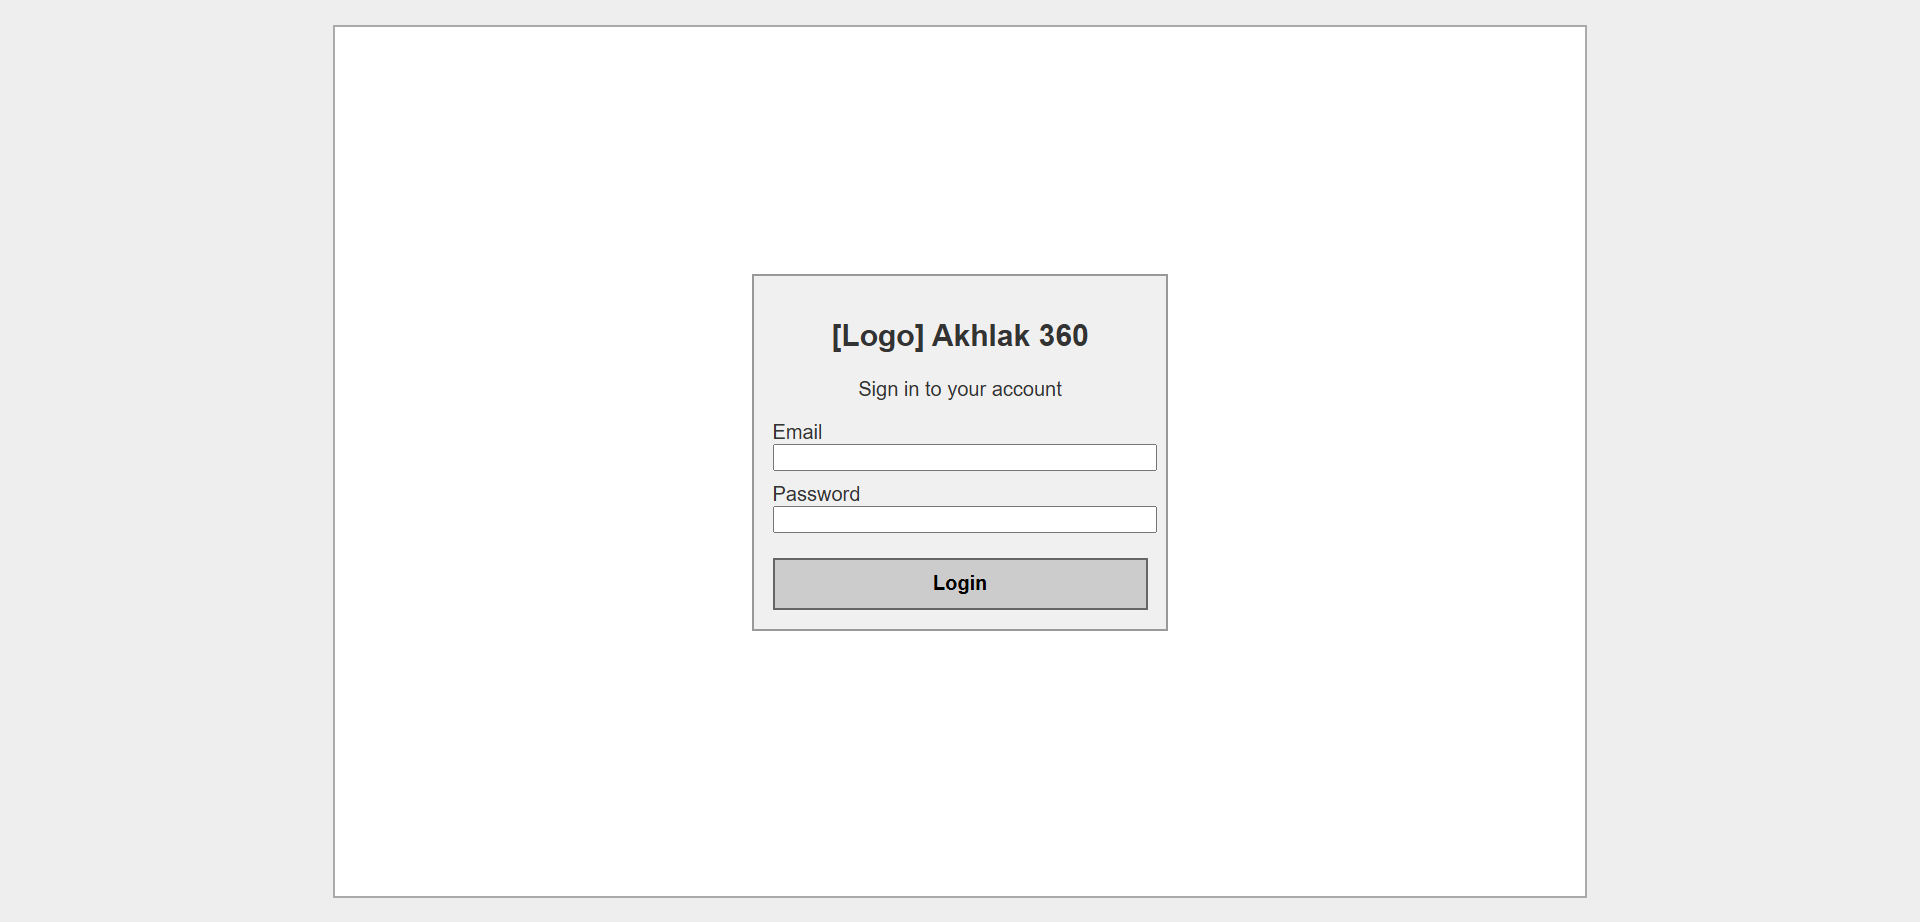
\includegraphics[width=0.8\textwidth]{lofi-login.png}
  \caption{Lo-Fi: Halaman Login}
\end{figure}

\begin{figure}[H]
  \centering
  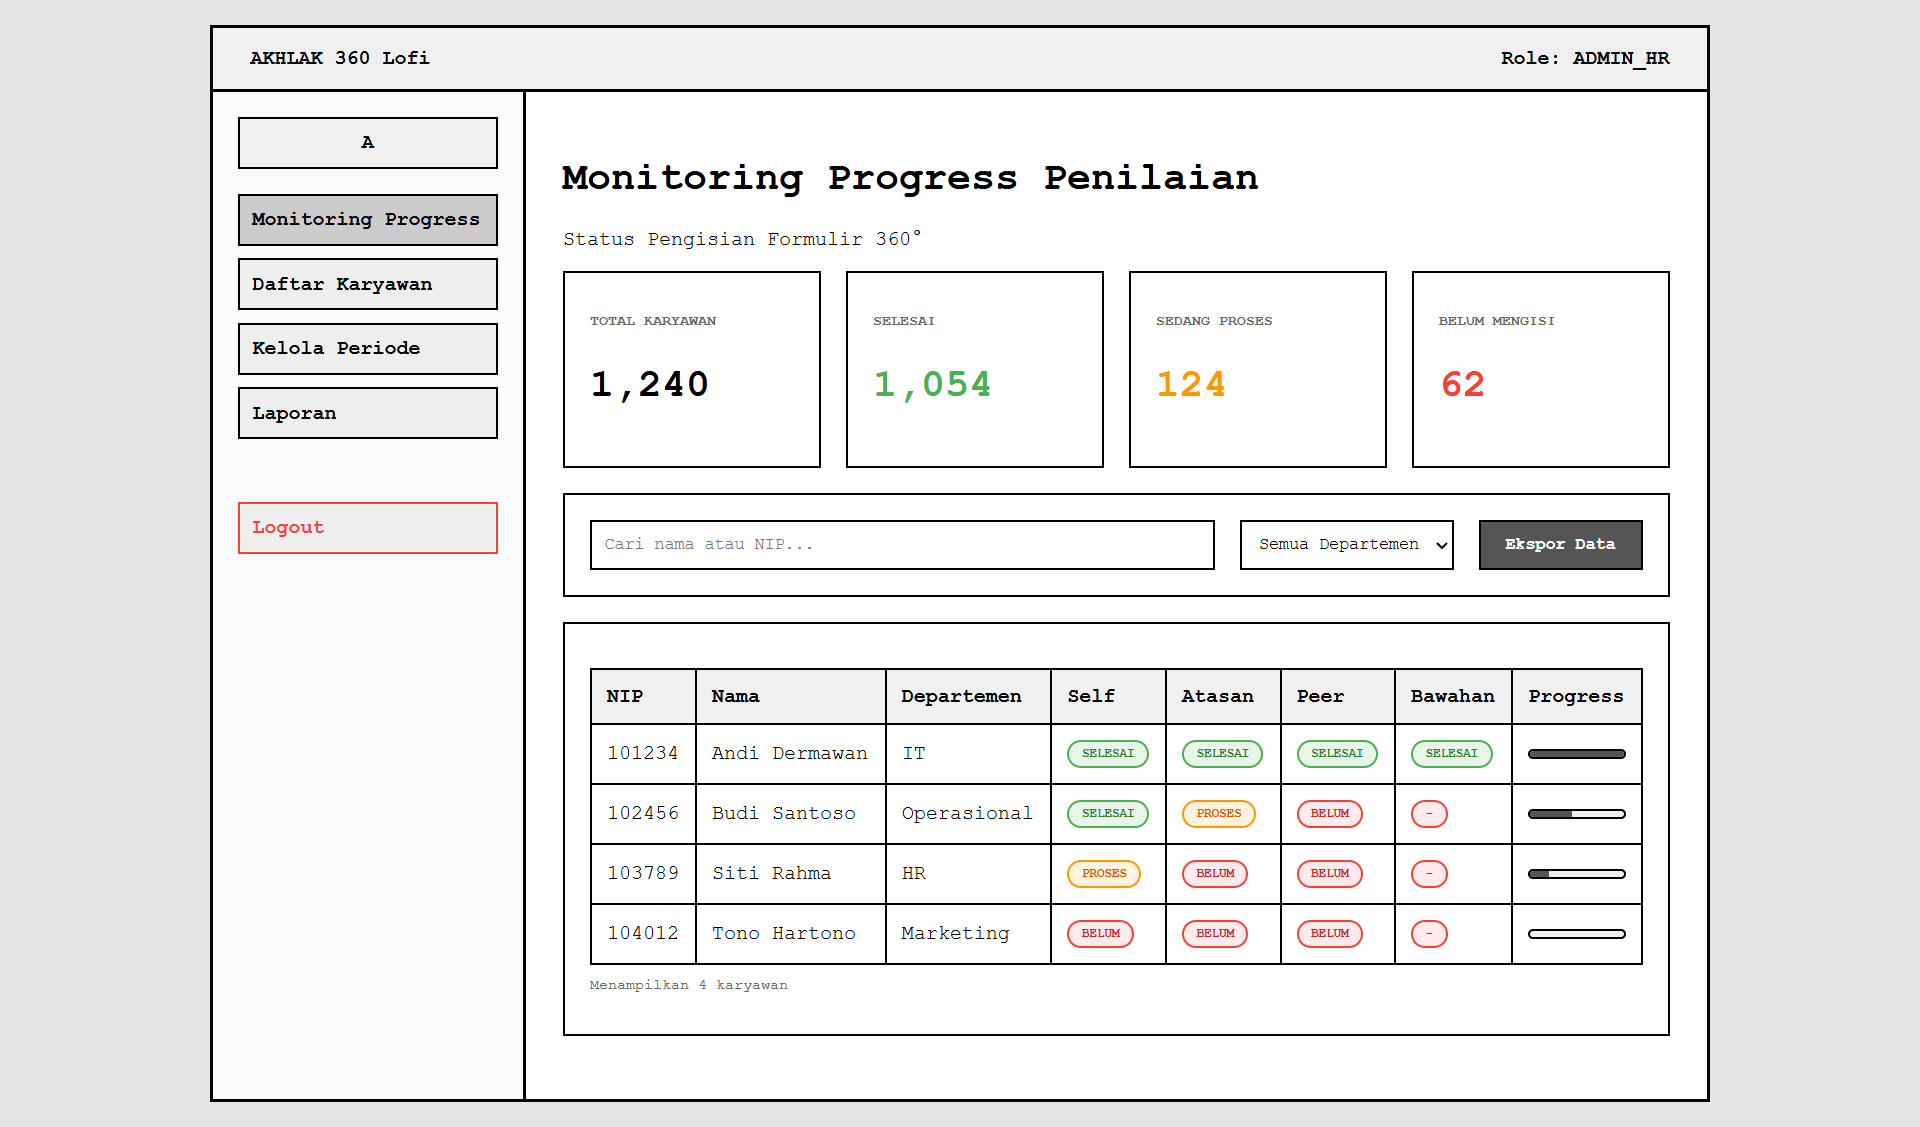
\includegraphics[width=0.8\textwidth]{lofi-dashboard-admin.png}
  \caption{Lo-Fi: Dashboard Admin HR -- Monitoring Progress}
\end{figure}

\begin{figure}[H]
  \centering
  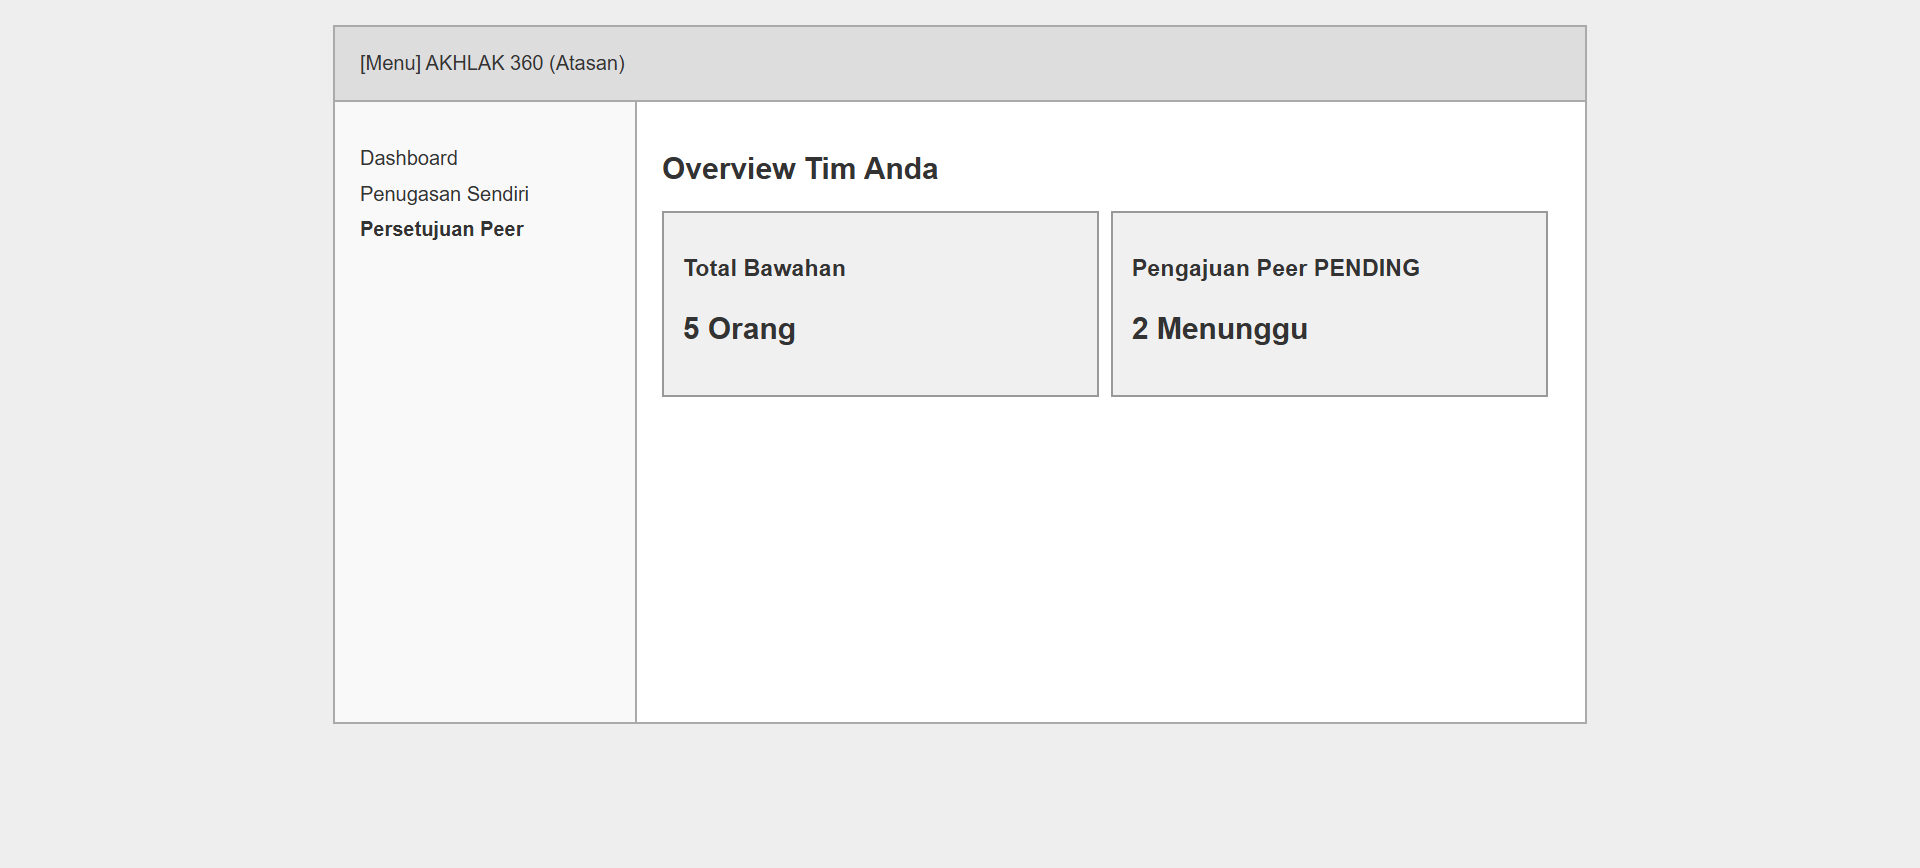
\includegraphics[width=0.8\textwidth]{lofi-dashboard-atasan.png}
  \caption{Lo-Fi: Dashboard Atasan -- Dashboard Tim}
\end{figure}

\begin{figure}[H]
  \centering
  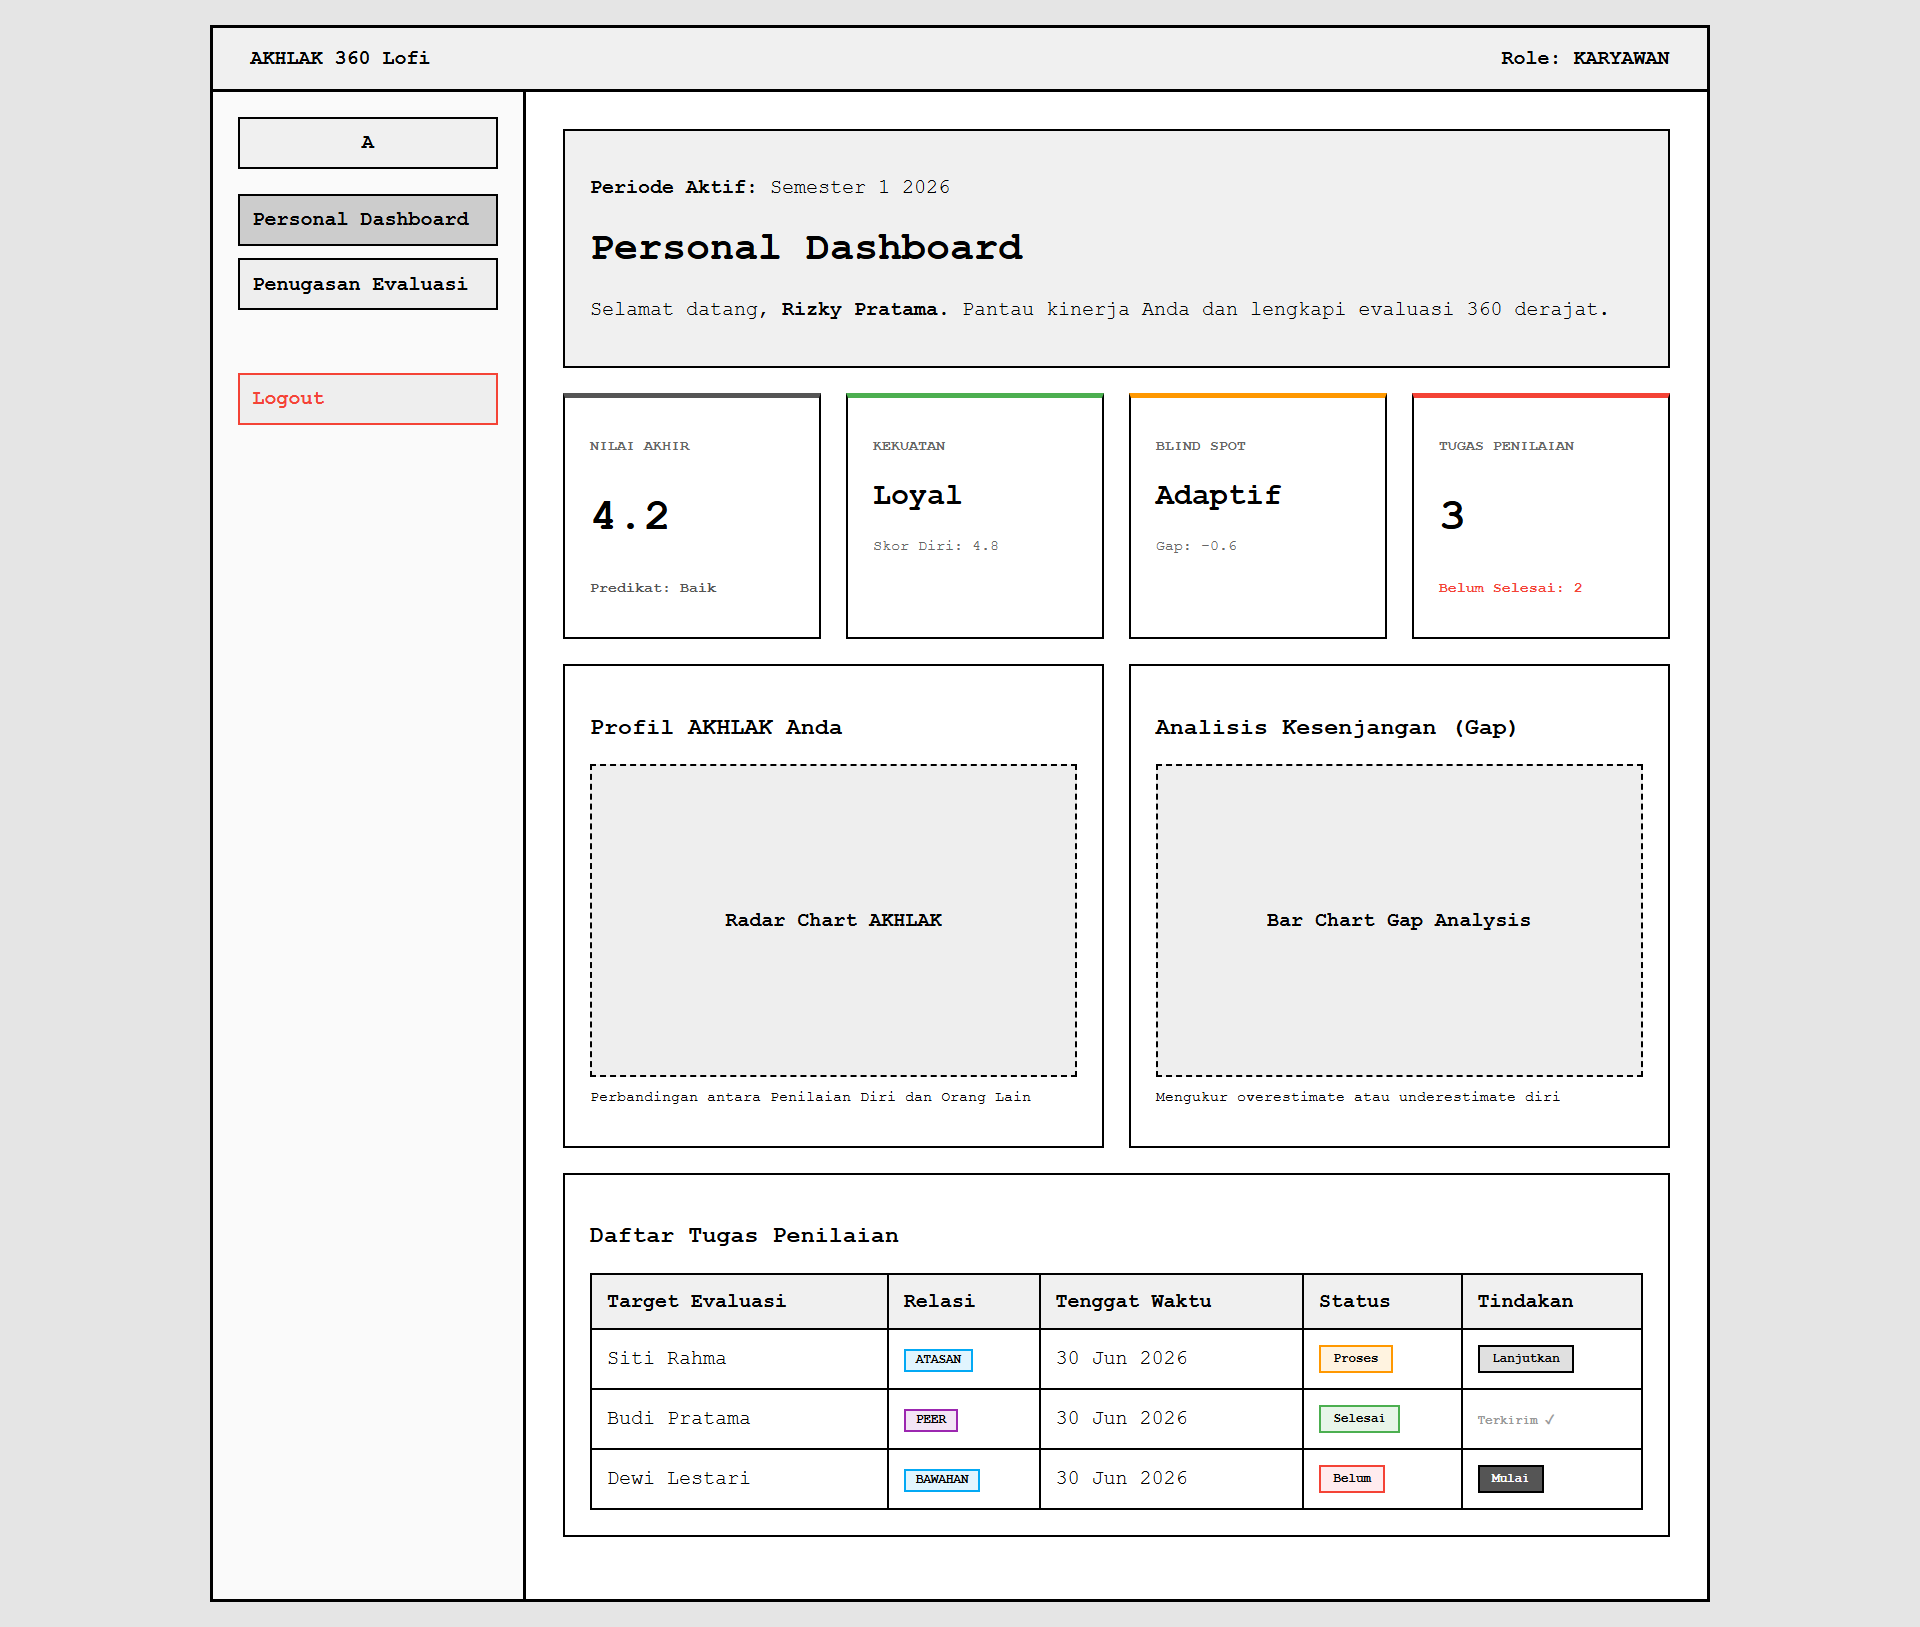
\includegraphics[width=0.8\textwidth]{lofi-dashboard-karyawan.png}
  \caption{Lo-Fi: Dashboard Karyawan -- Personal Dashboard}
\end{figure}

\begin{figure}[H]
  \centering
  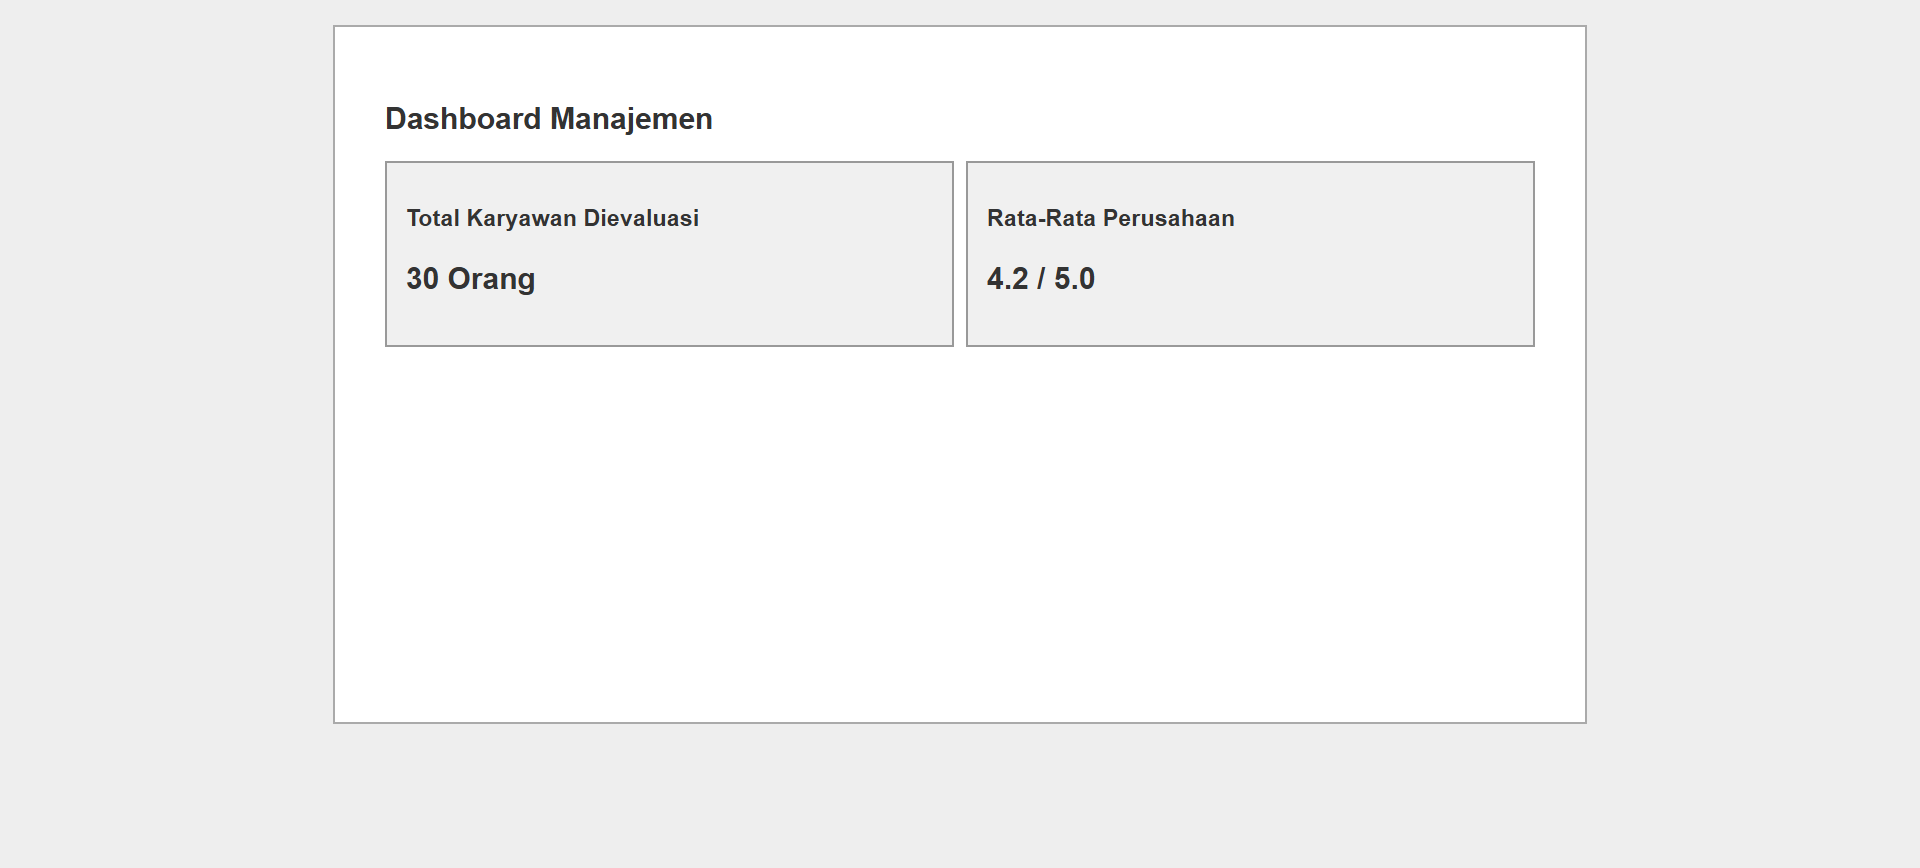
\includegraphics[width=0.8\textwidth]{lofi-dashboard-manajemen.png}
  \caption{Lo-Fi: Dashboard Manajemen -- Executive Dashboard}
\end{figure}

\begin{figure}[H]
  \centering
  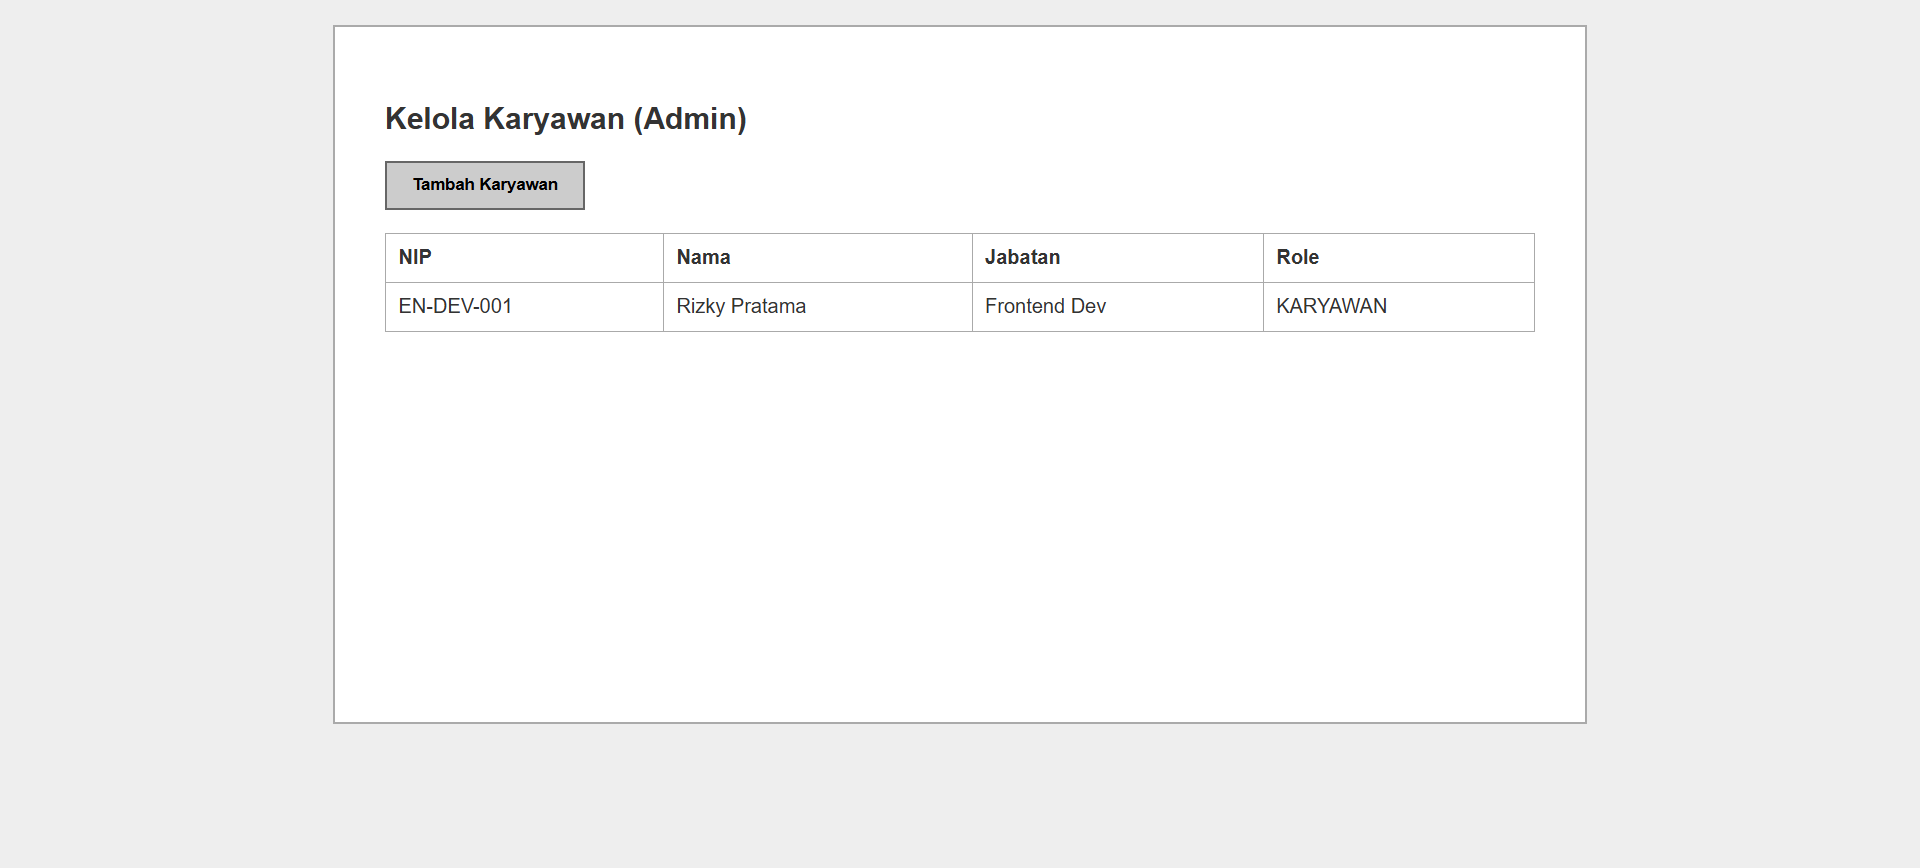
\includegraphics[width=0.8\textwidth]{lofi-kelola-karyawan.png}
  \caption{Lo-Fi: Kelola Data Karyawan (Admin HR)}
\end{figure}

\begin{figure}[H]
  \centering
  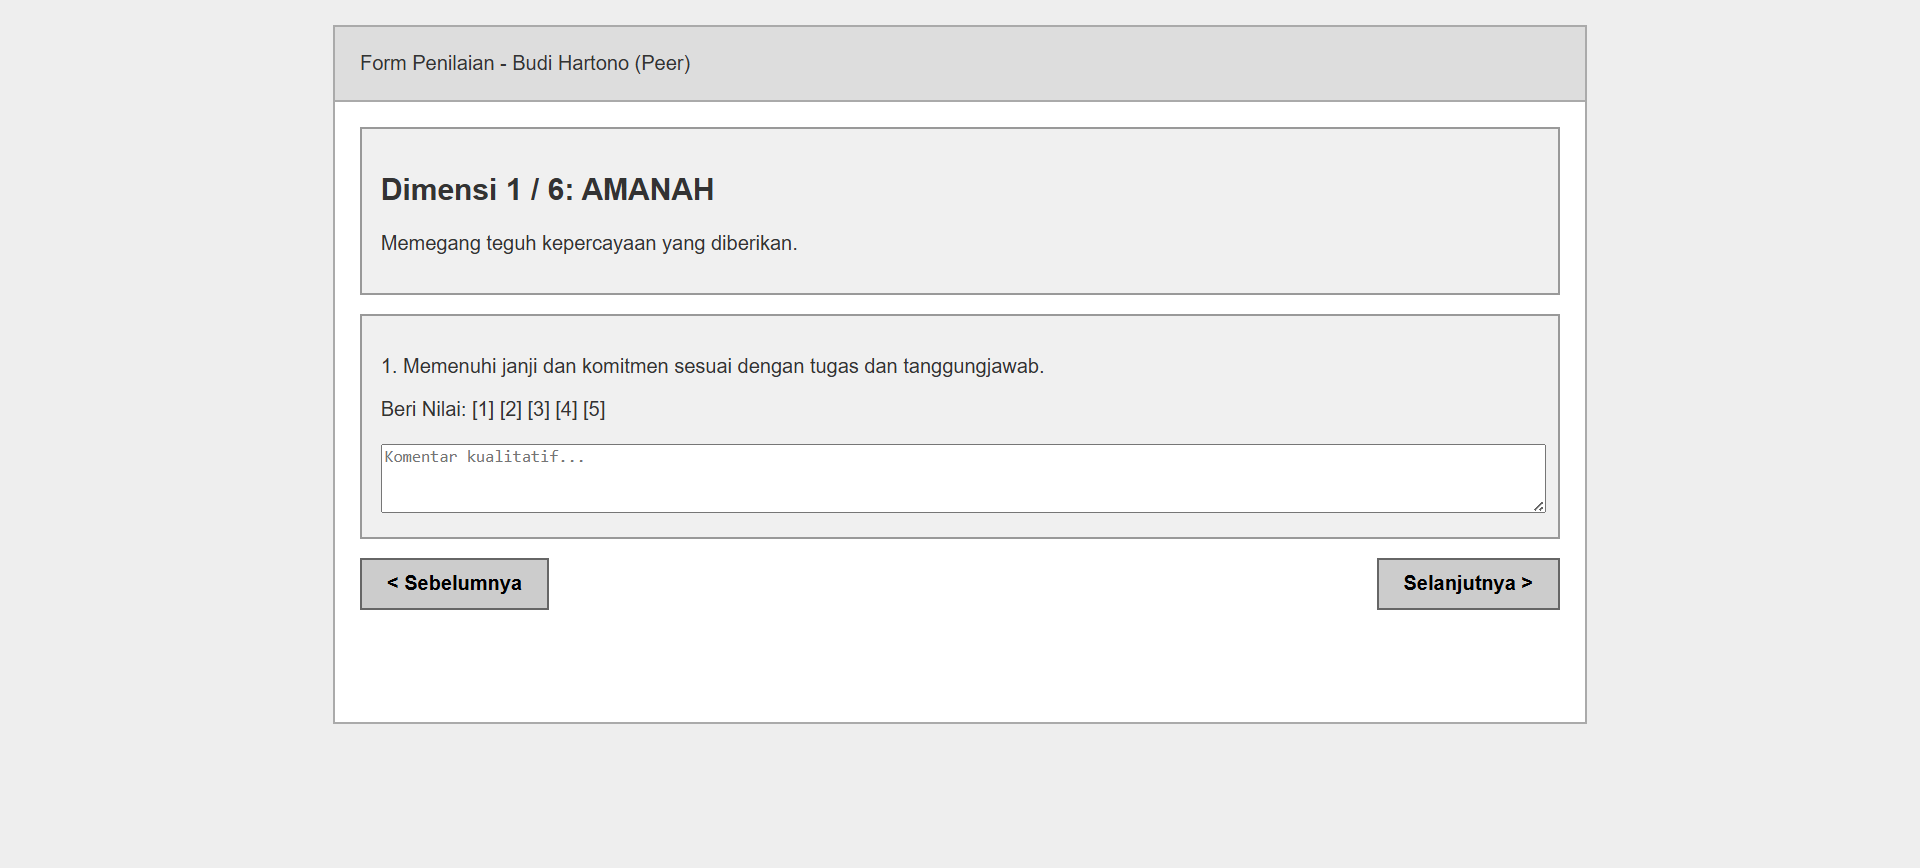
\includegraphics[width=0.8\textwidth]{lofi-form-penilaian.png}
  \caption{Lo-Fi: Form Penilaian 360\textdegree{} (Wizard dengan Star Rating)}
\end{figure}

\begin{figure}[H]
  \centering
  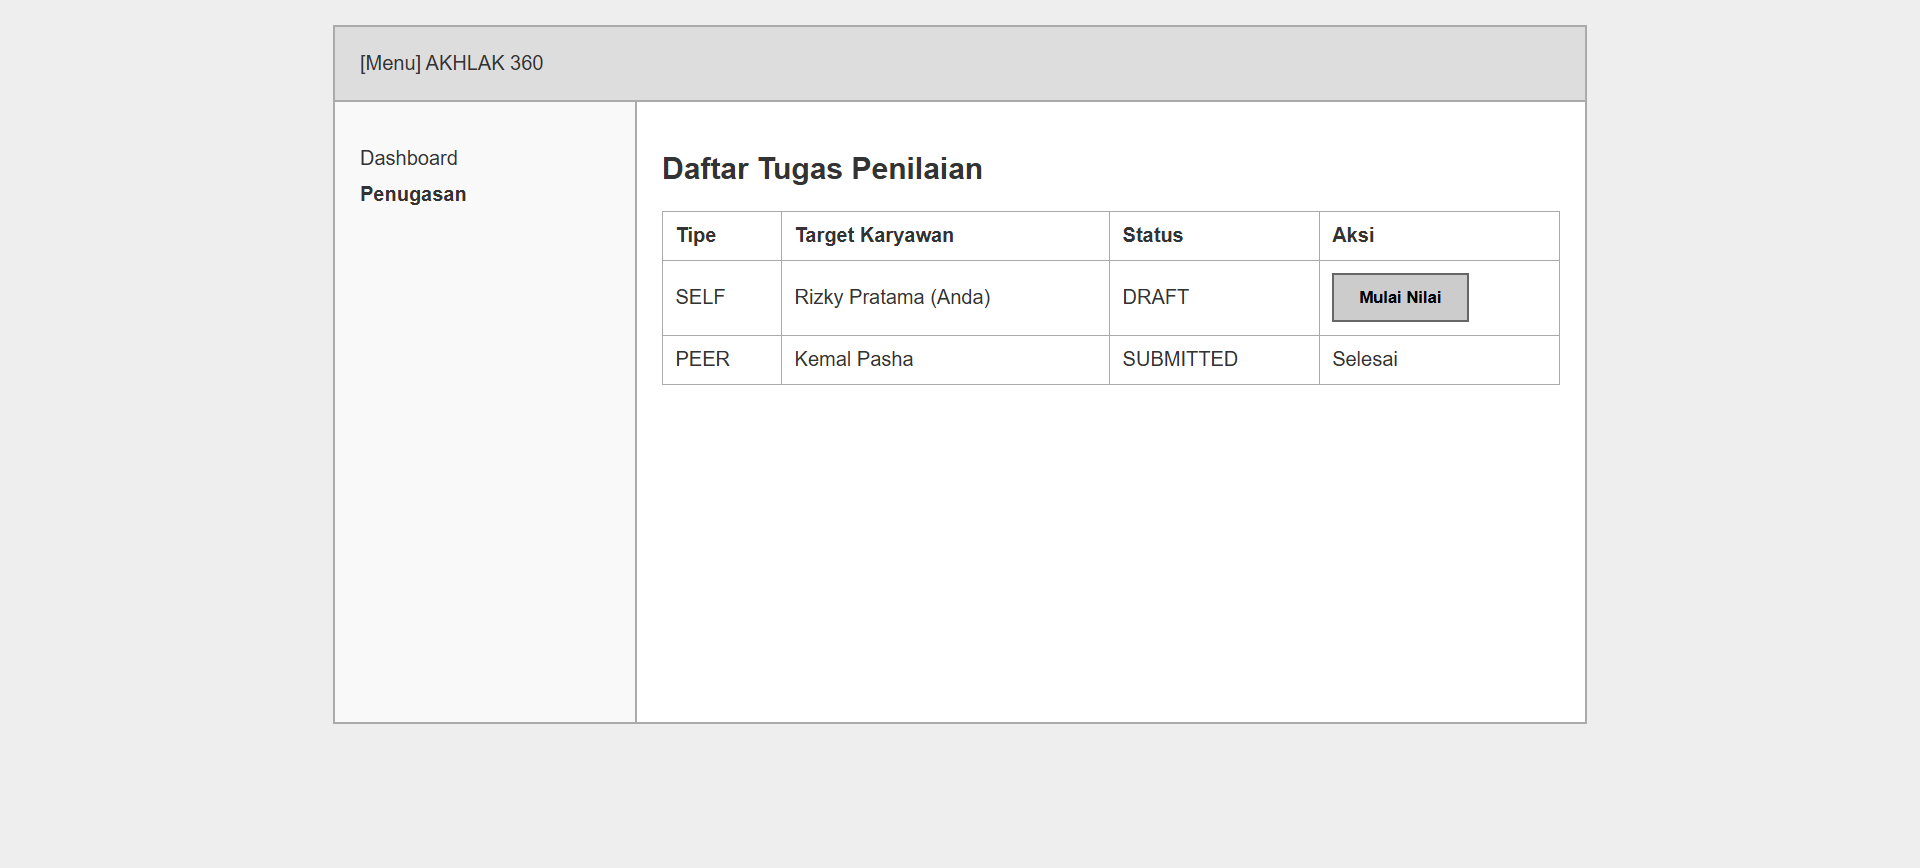
\includegraphics[width=0.8\textwidth]{lofi-penugasan-karyawan.png}
  \caption{Lo-Fi: Penugasan Evaluasi Karyawan}
\end{figure}

\begin{figure}[H]
  \centering
  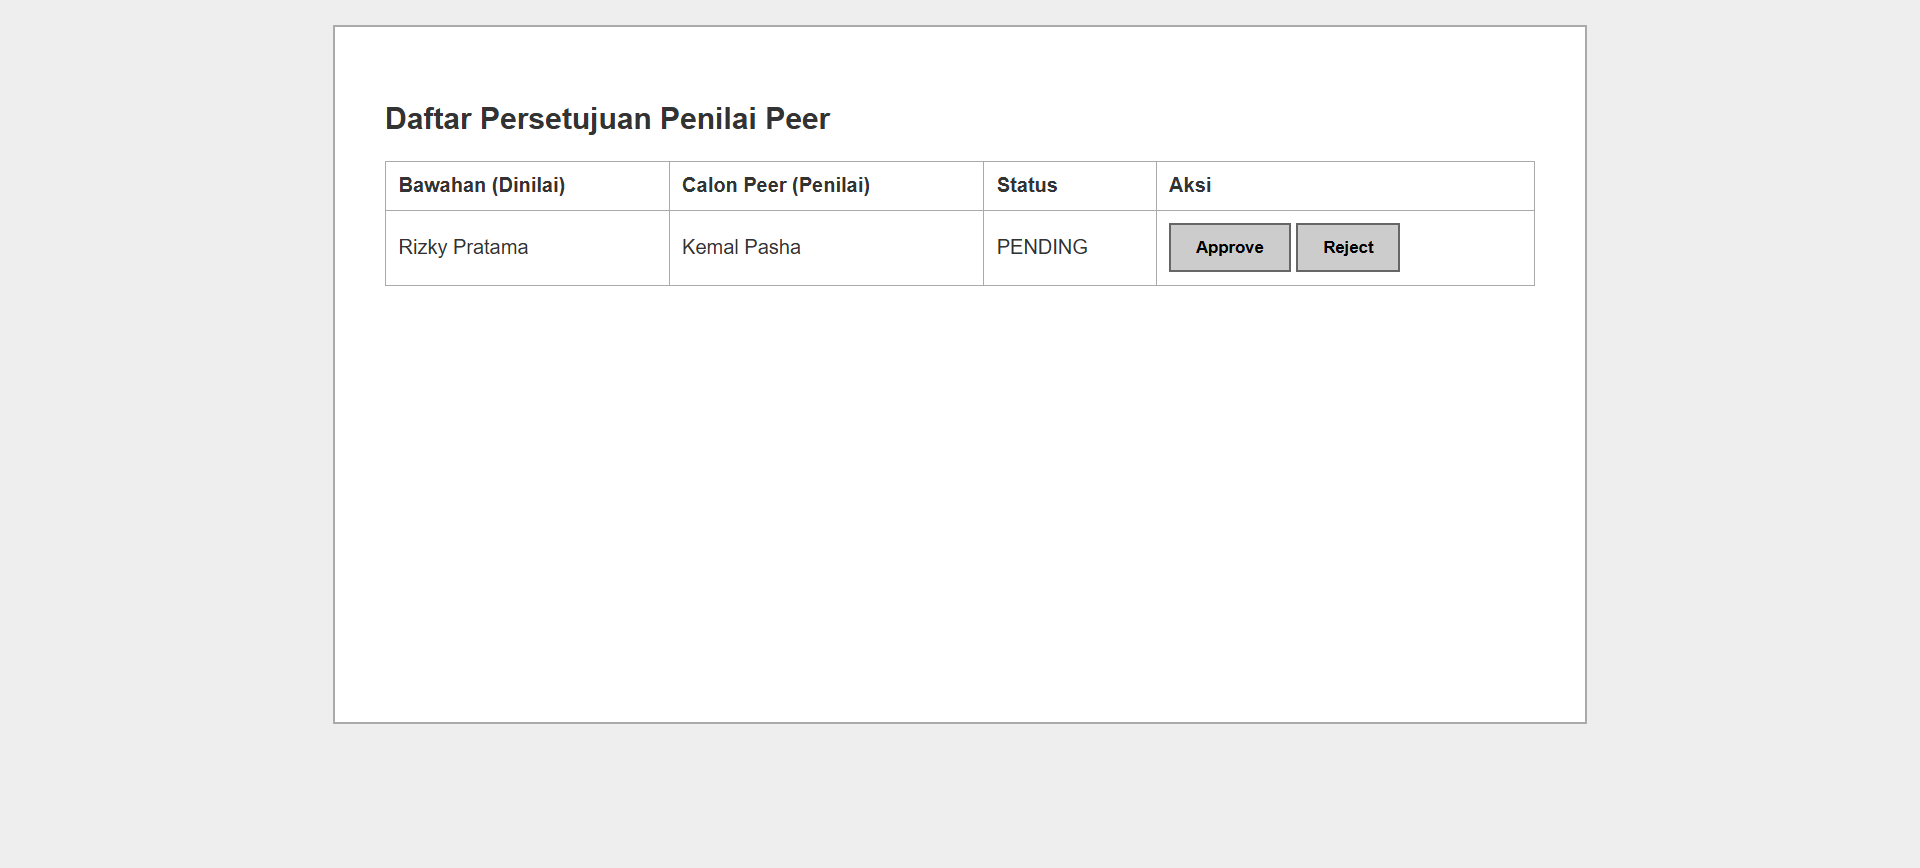
\includegraphics[width=0.8\textwidth]{lofi-persetujuan-peer.png}
  \caption{Lo-Fi: Persetujuan Daftar Peer (Atasan)}
\end{figure}

\begin{figure}[H]
  \centering
  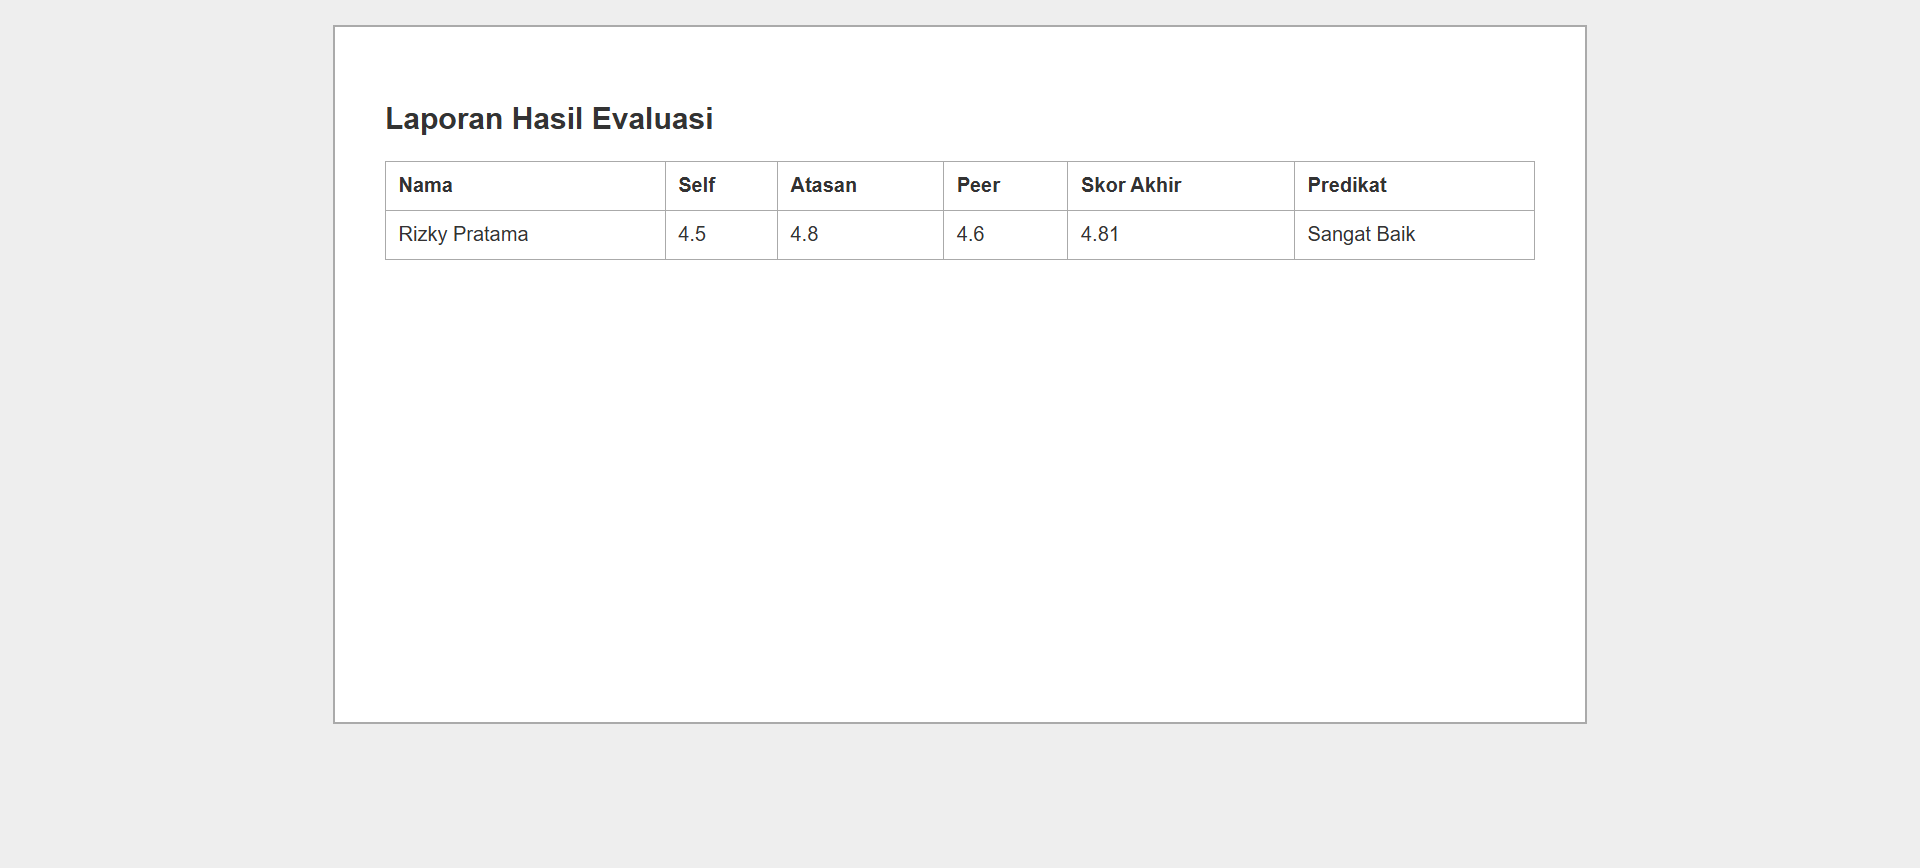
\includegraphics[width=0.8\textwidth]{lofi-laporan-akhir.png}
  \caption{Lo-Fi: Laporan Akhir Evaluasi}
\end{figure}

\begin{figure}[H]
  \centering
  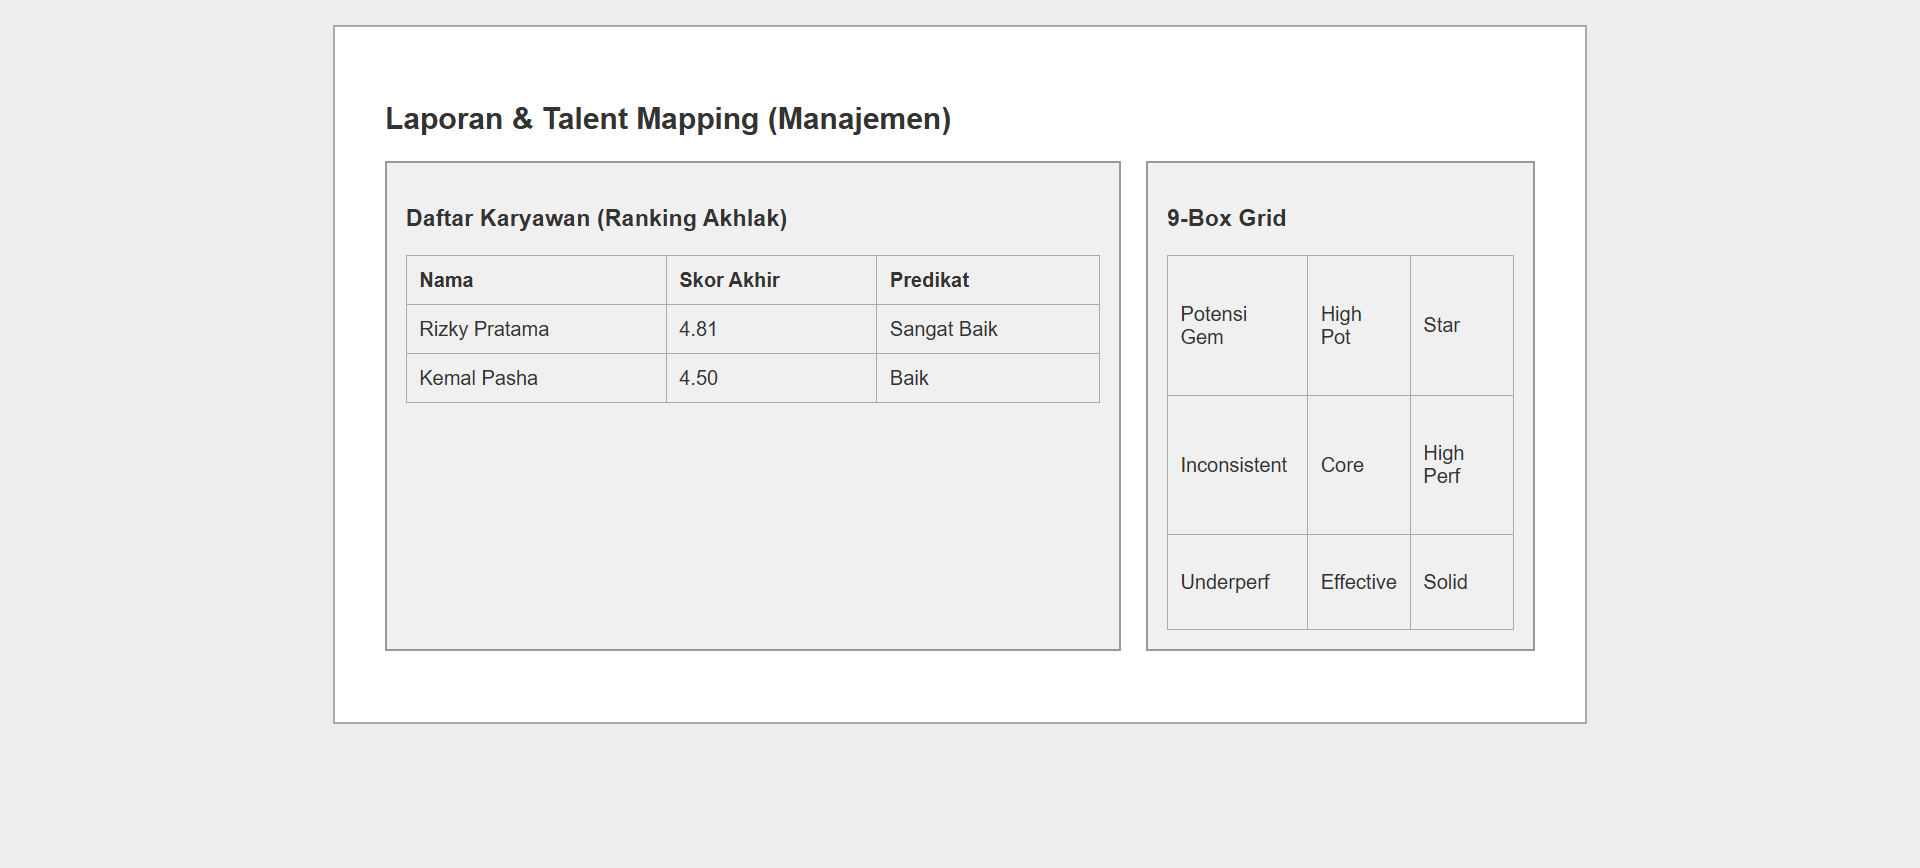
\includegraphics[width=0.8\textwidth]{lofi-laporan-9box.png}
  \caption{Lo-Fi: 9-Box Talent Mapping}
\end{figure}

\newpage
\section{High Fidelity Prototype}

Berikut adalah \textit{high fidelity prototype} dari sistem informasi penilaian 360\textdegree{} Core Values AKHLAK. Prototype ini dirancang menggunakan \textit{framework} Tailwind CSS dengan skema warna biru (\textit{brand}) dan putih, mencerminkan identitas korporat PT Energi Nusantara.

\begin{figure}[H]
  \centering
  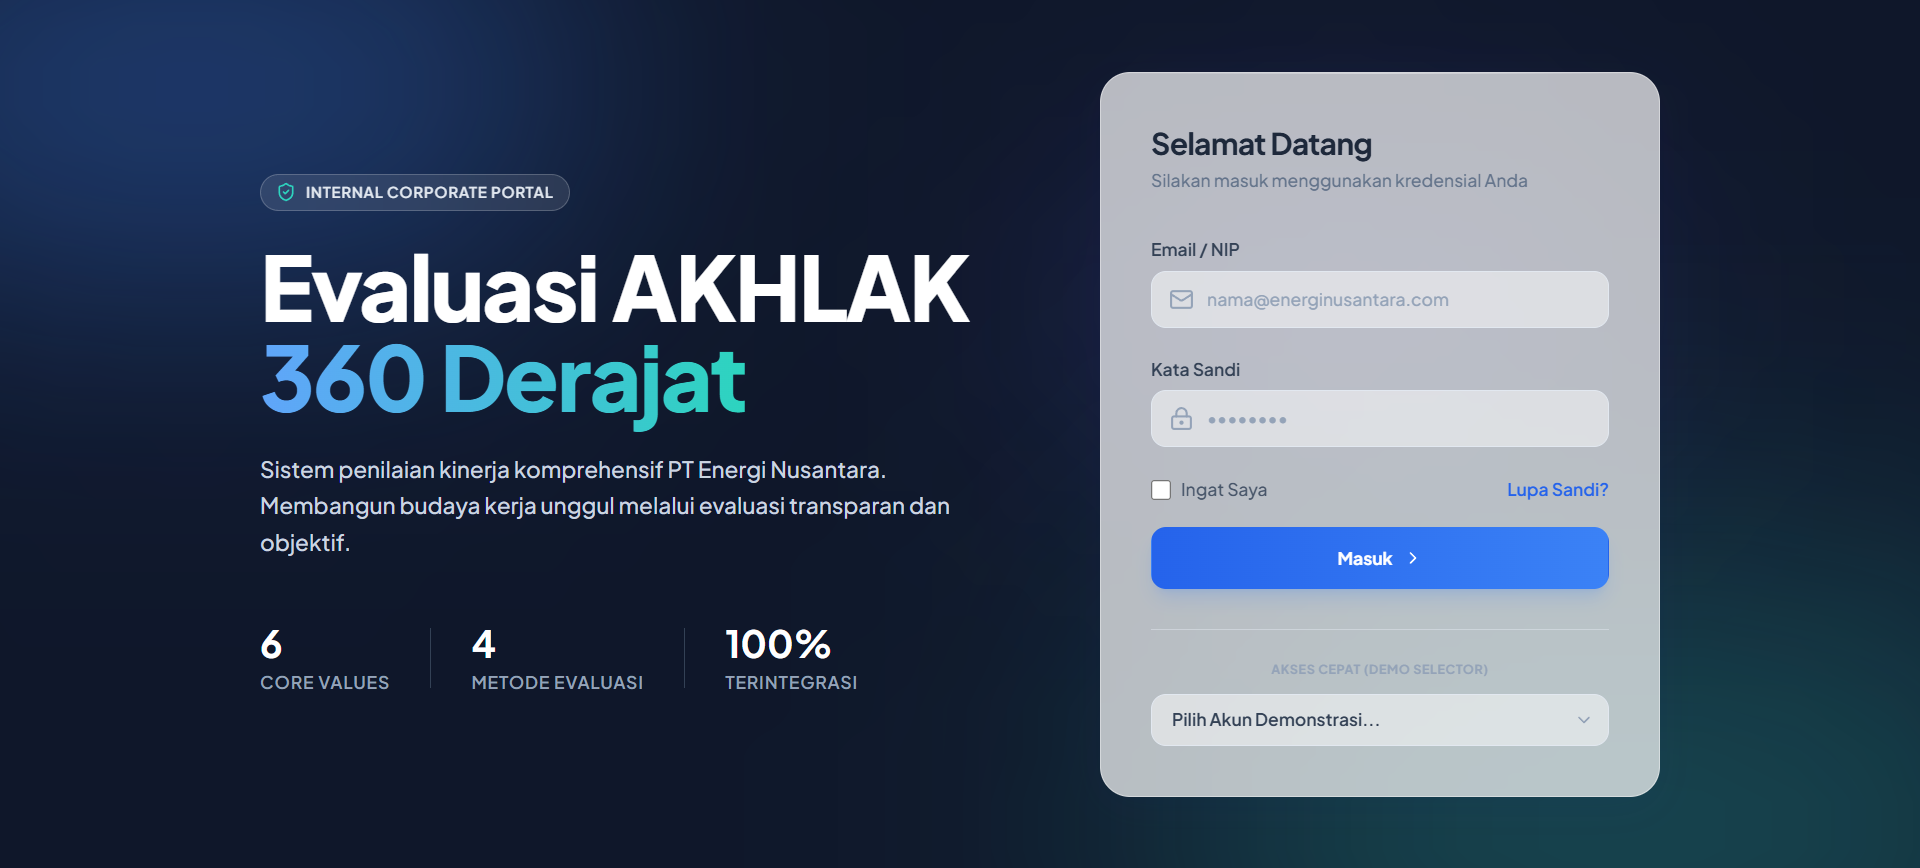
\includegraphics[width=0.8\textwidth]{hifi-login.png}
  \caption{Hi-Fi: Halaman Login dengan Demo Selector}
\end{figure}

\begin{figure}[H]
  \centering
  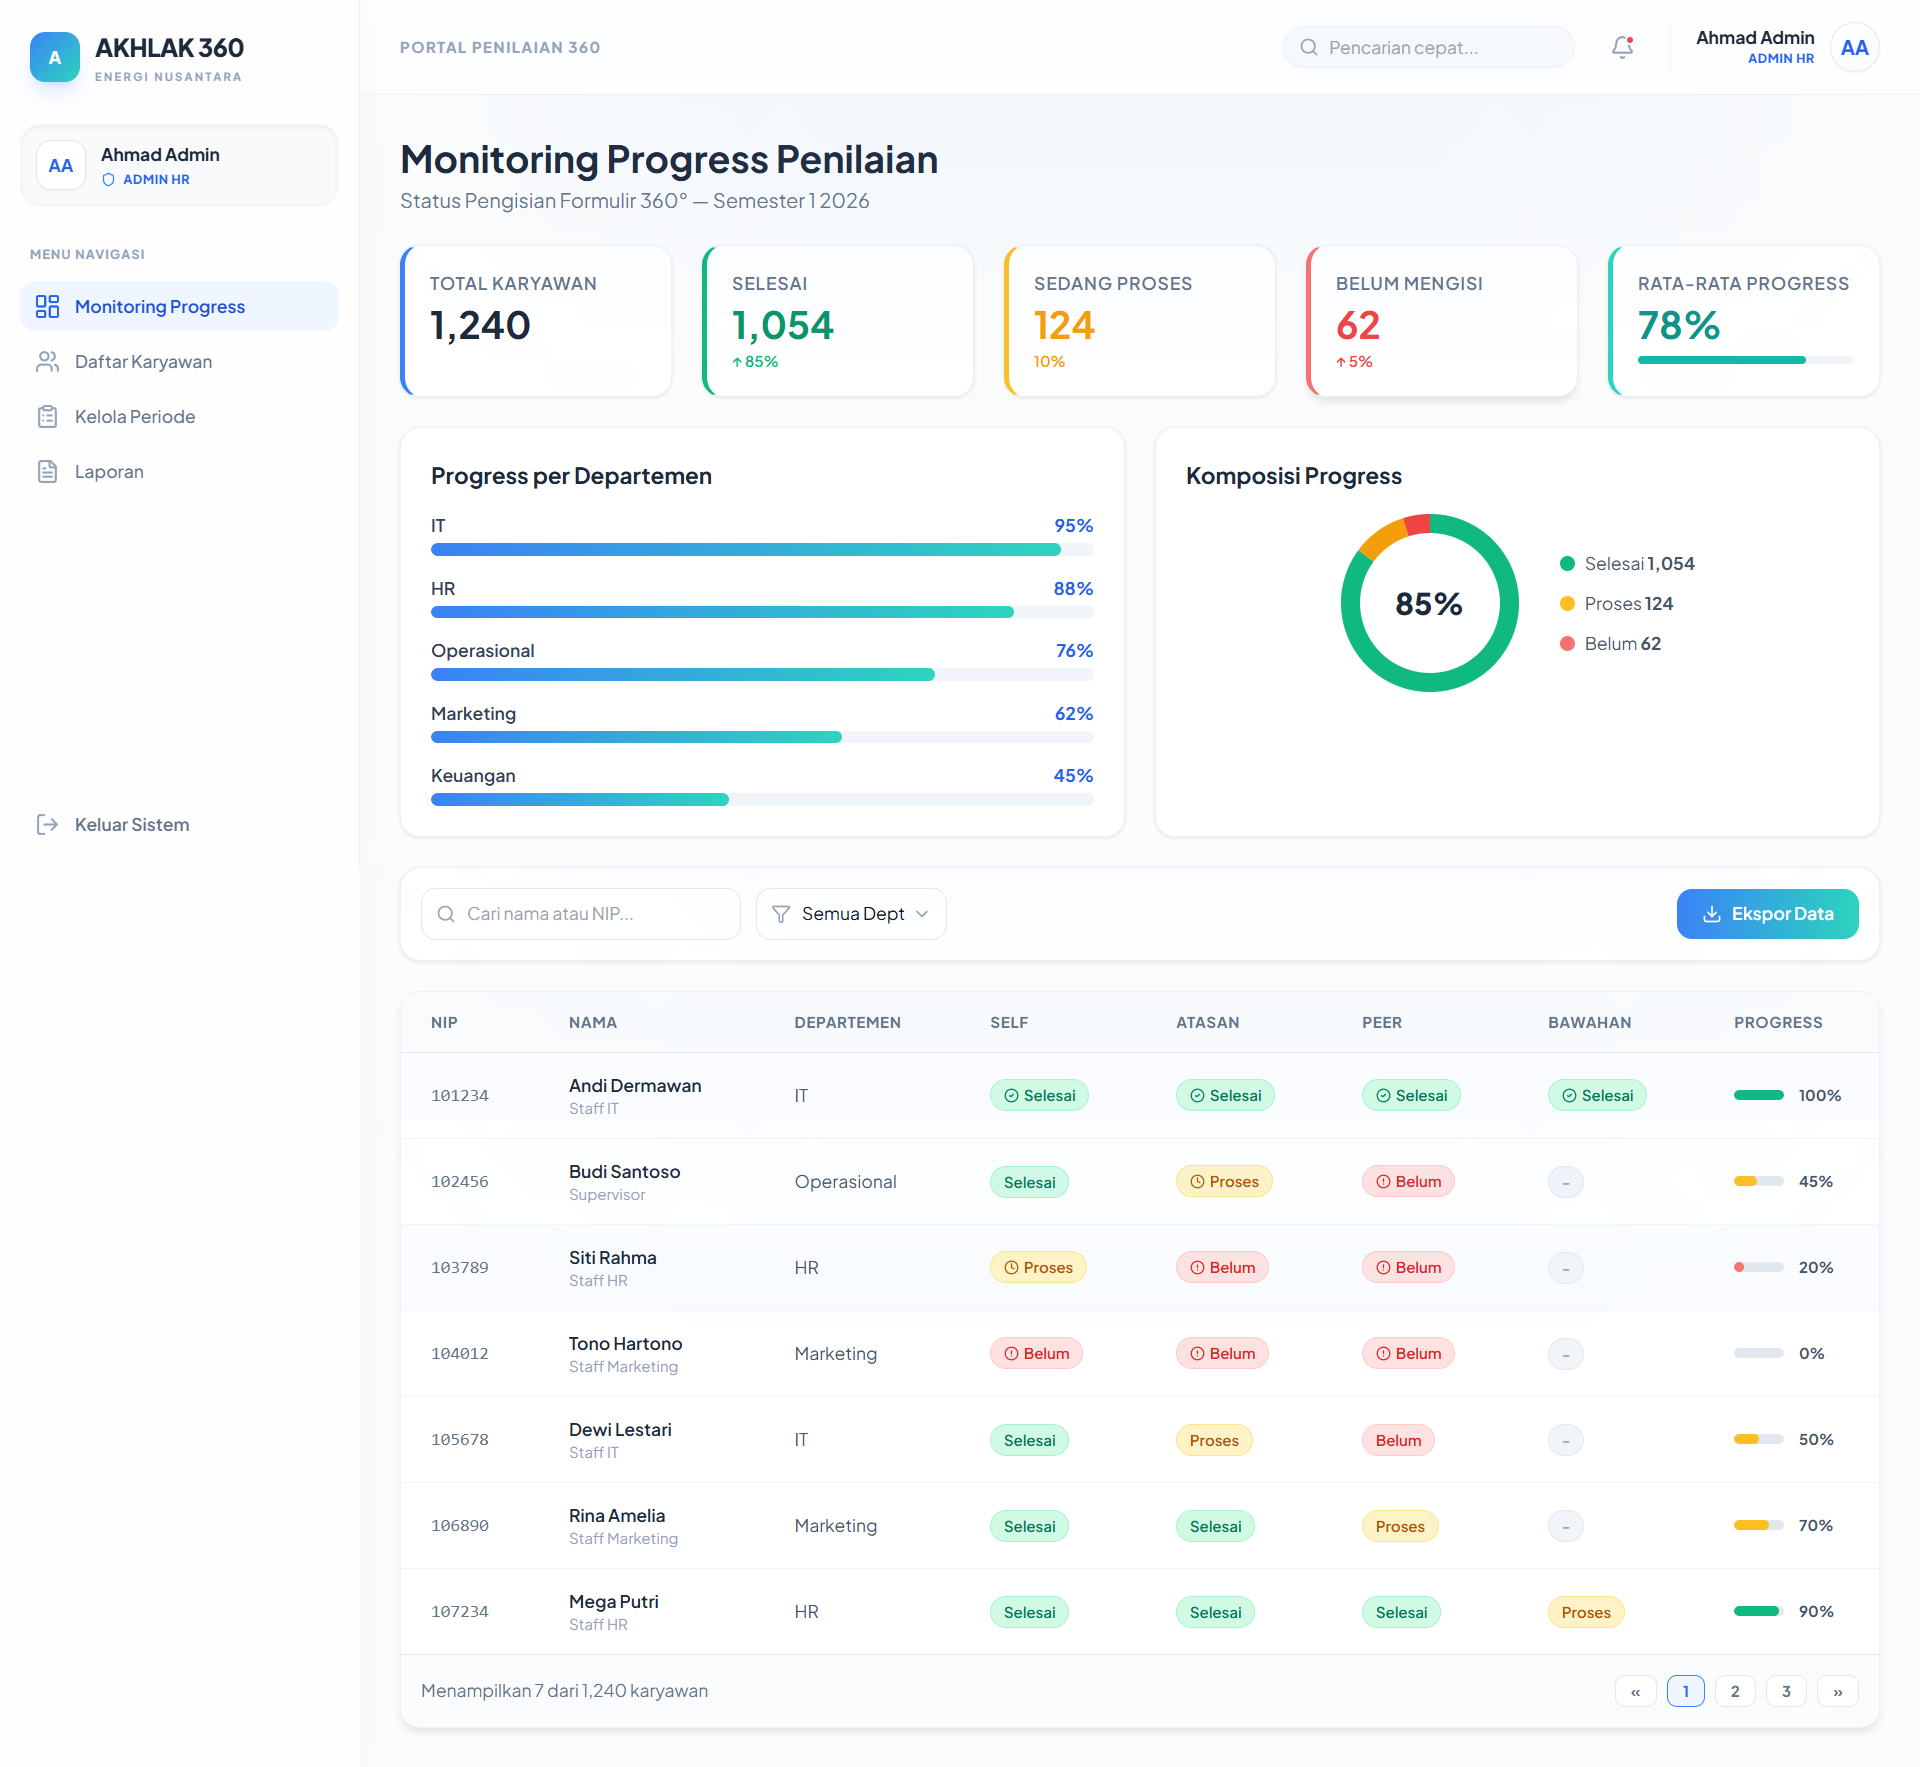
\includegraphics[width=0.8\textwidth]{hifi-dashboard-admin.png}
  \caption{Hi-Fi: Dashboard Admin HR -- Monitoring Progress}
\end{figure}

\begin{figure}[H]
  \centering
  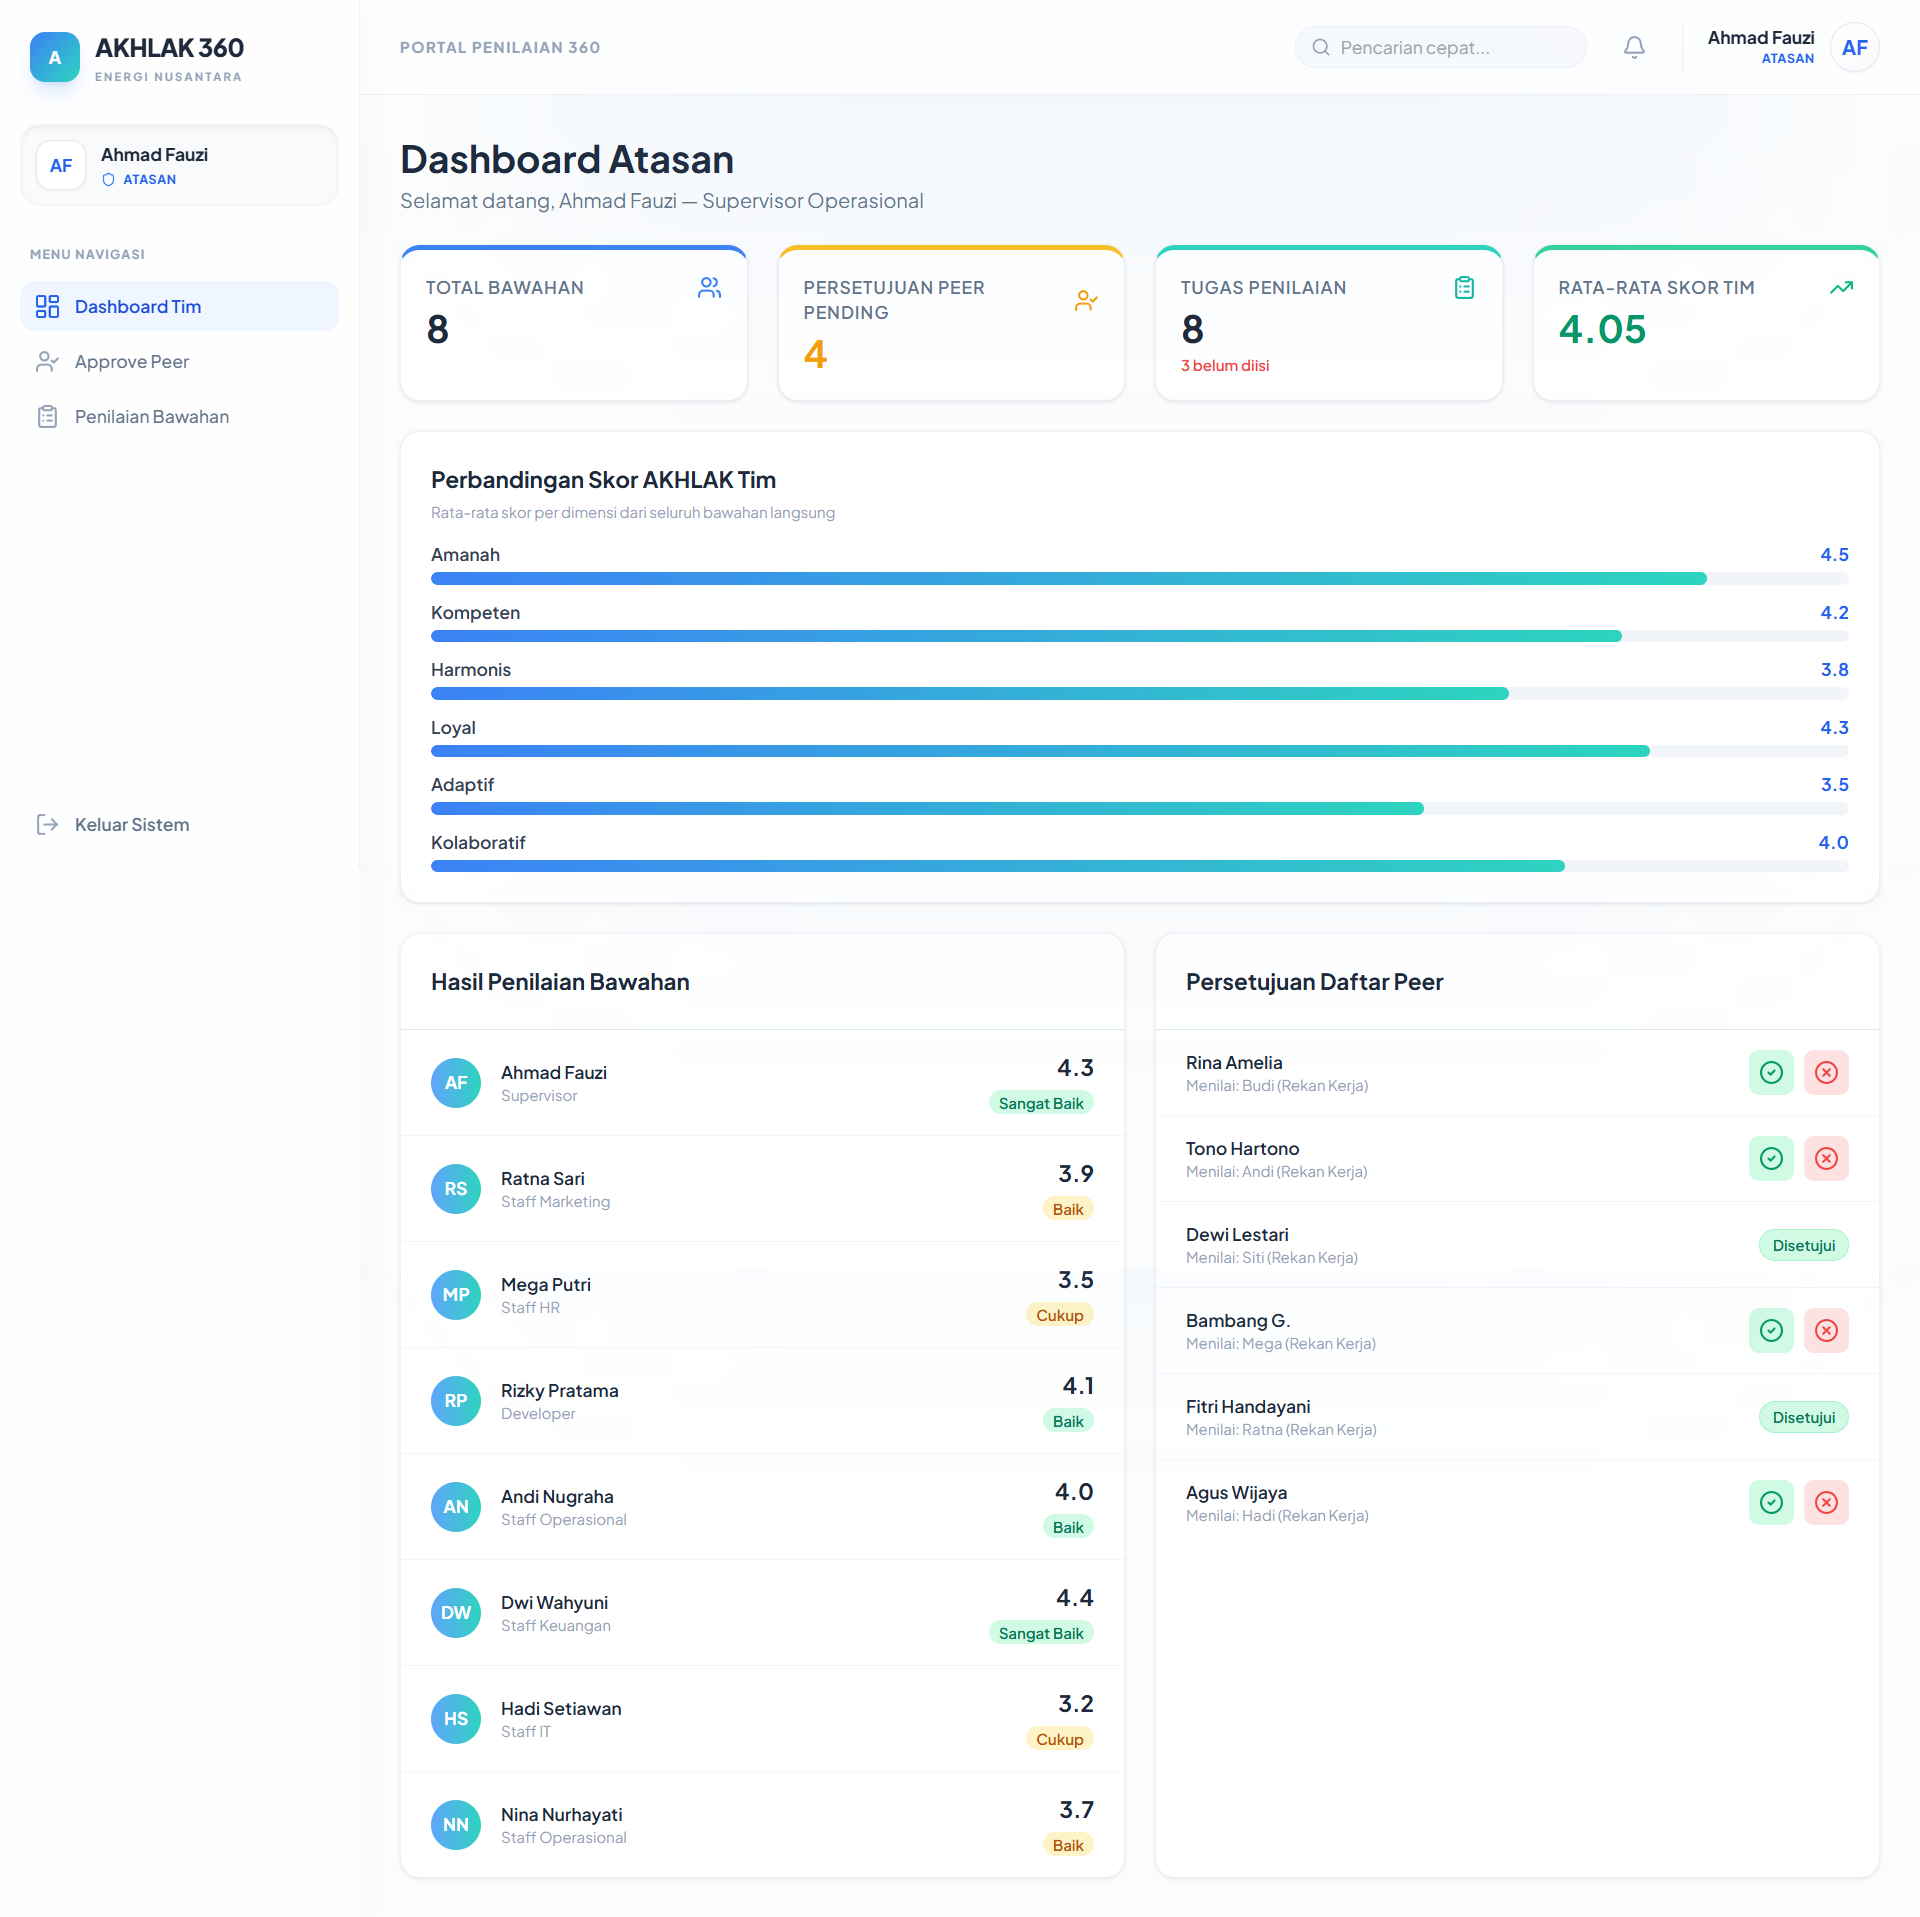
\includegraphics[width=0.8\textwidth]{hifi-dashboard-atasan.png}
  \caption{Hi-Fi: Dashboard Atasan -- Dashboard Tim}
\end{figure}

\begin{figure}[H]
  \centering
  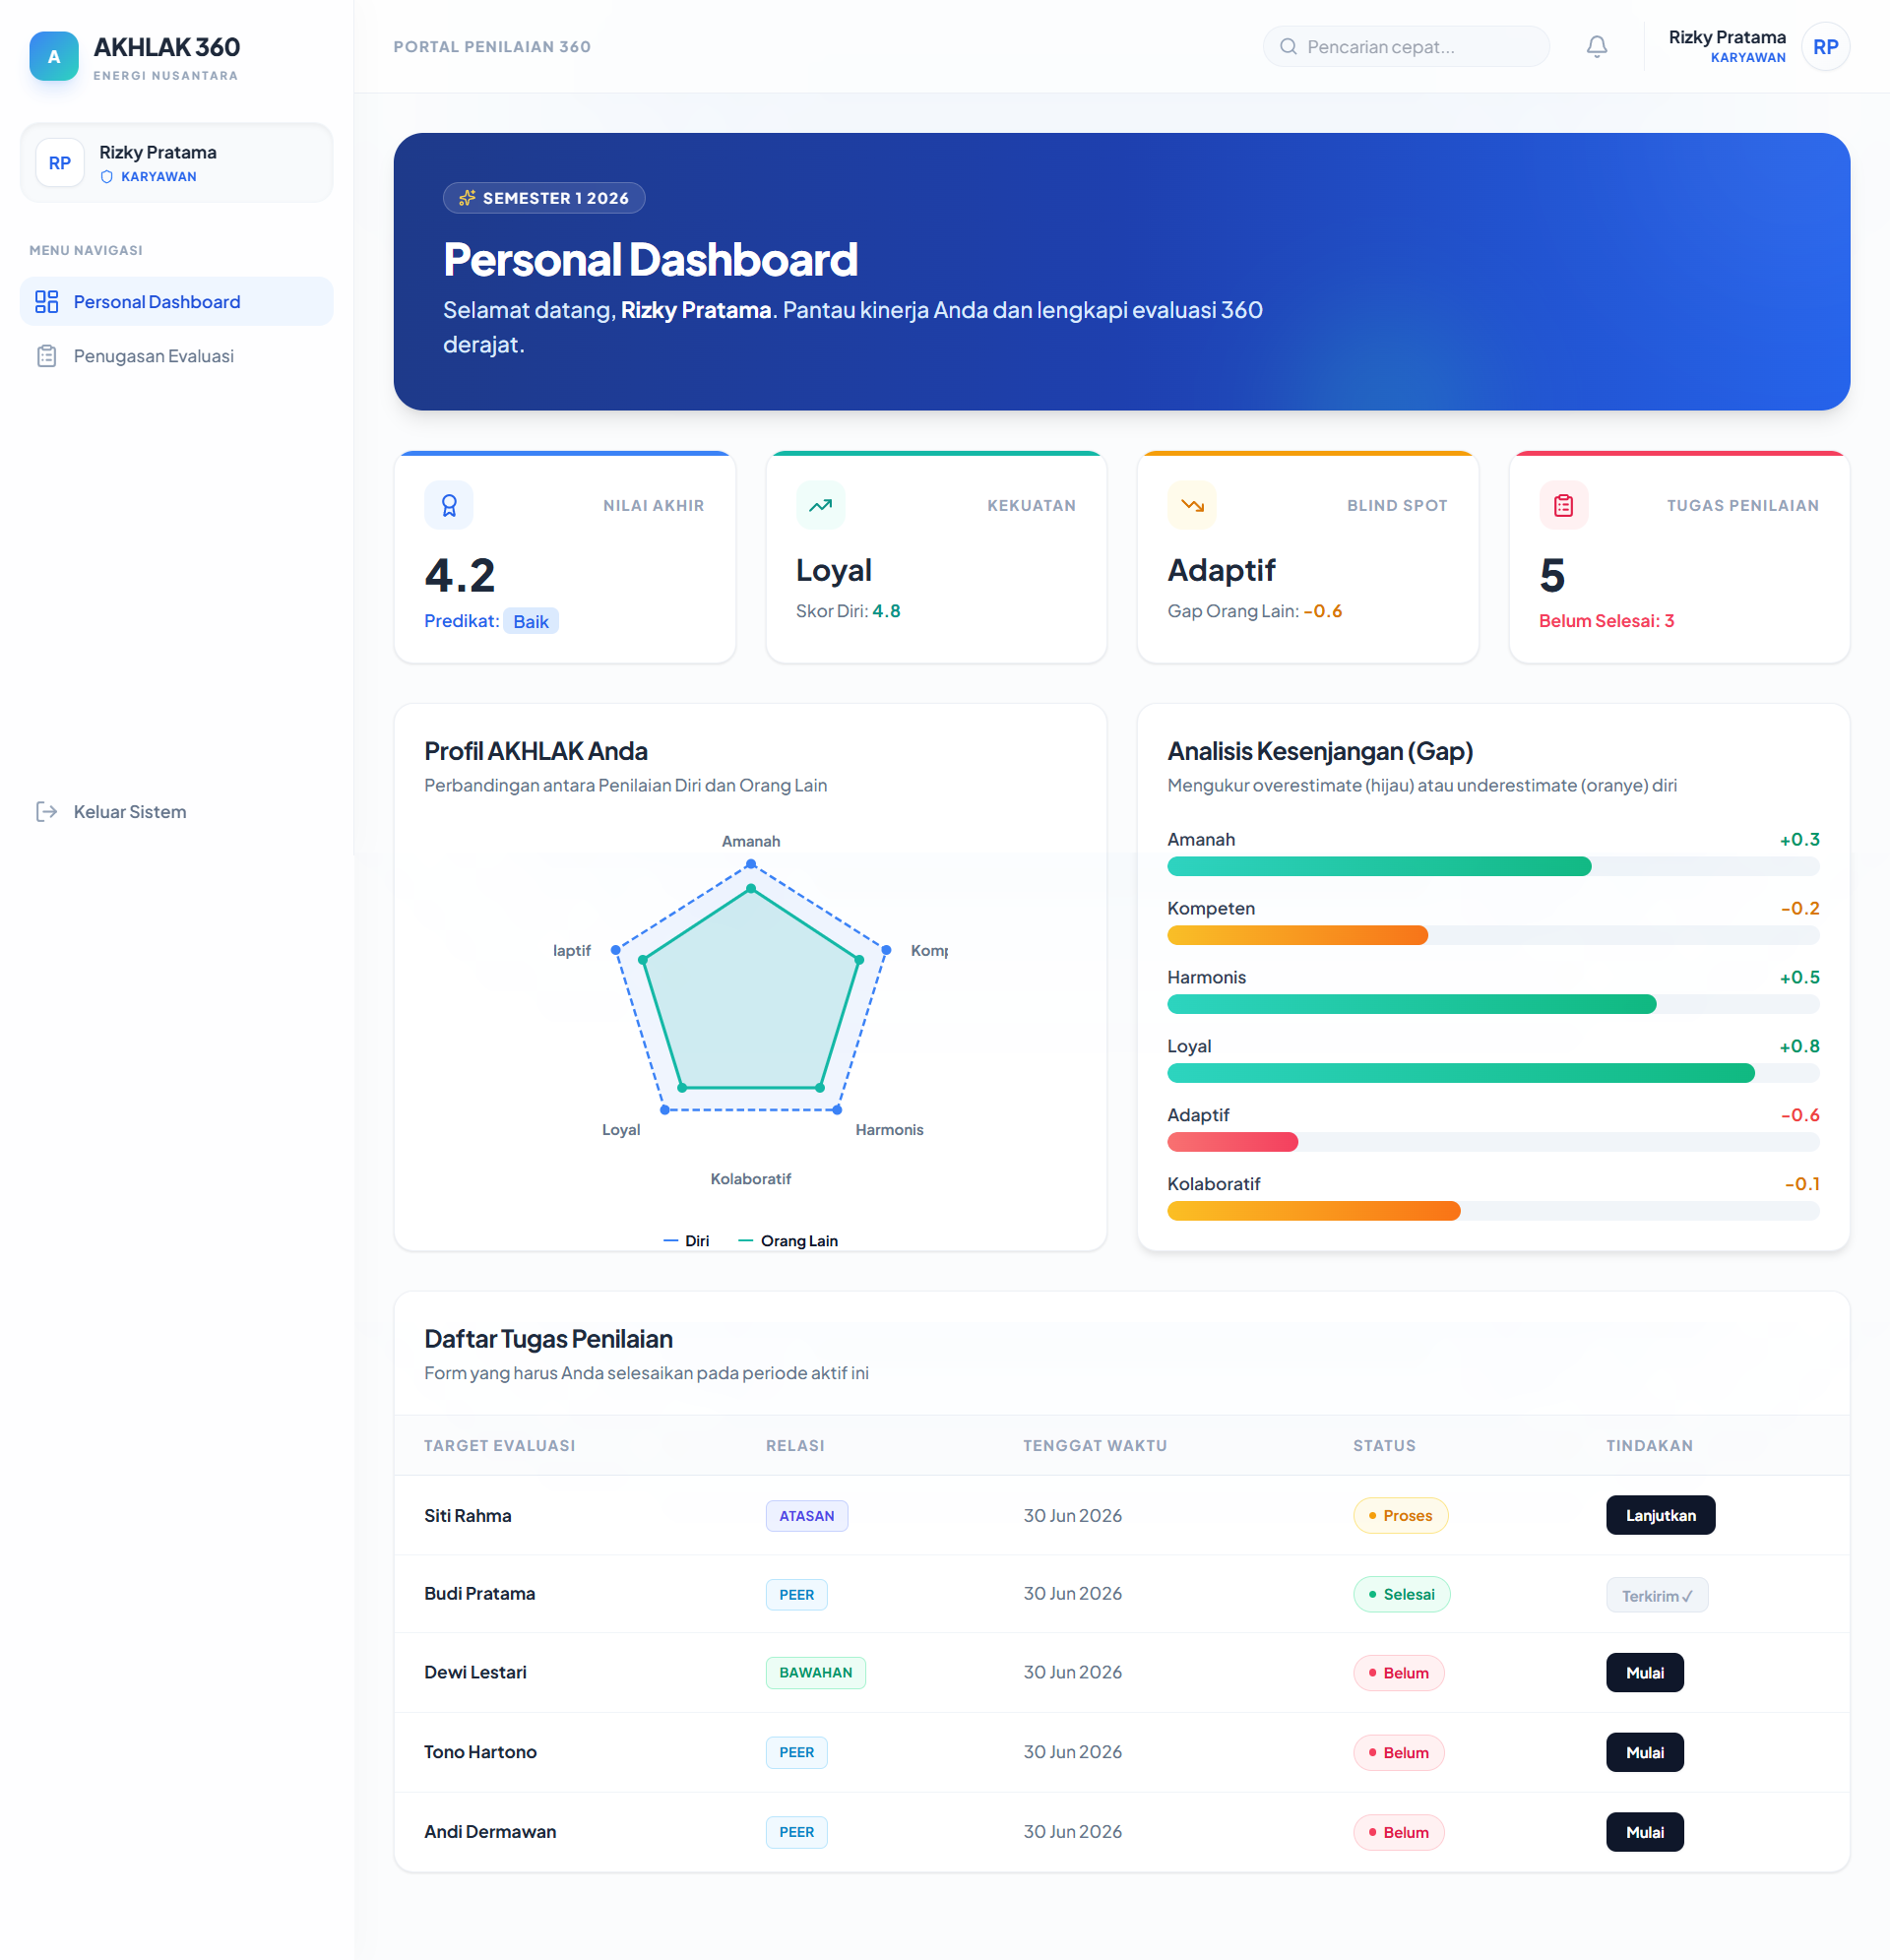
\includegraphics[width=0.8\textwidth]{hifi-dashboard-karyawan.png}
  \caption{Hi-Fi: Dashboard Karyawan -- Personal Dashboard}
\end{figure}

\begin{figure}[H]
  \centering
  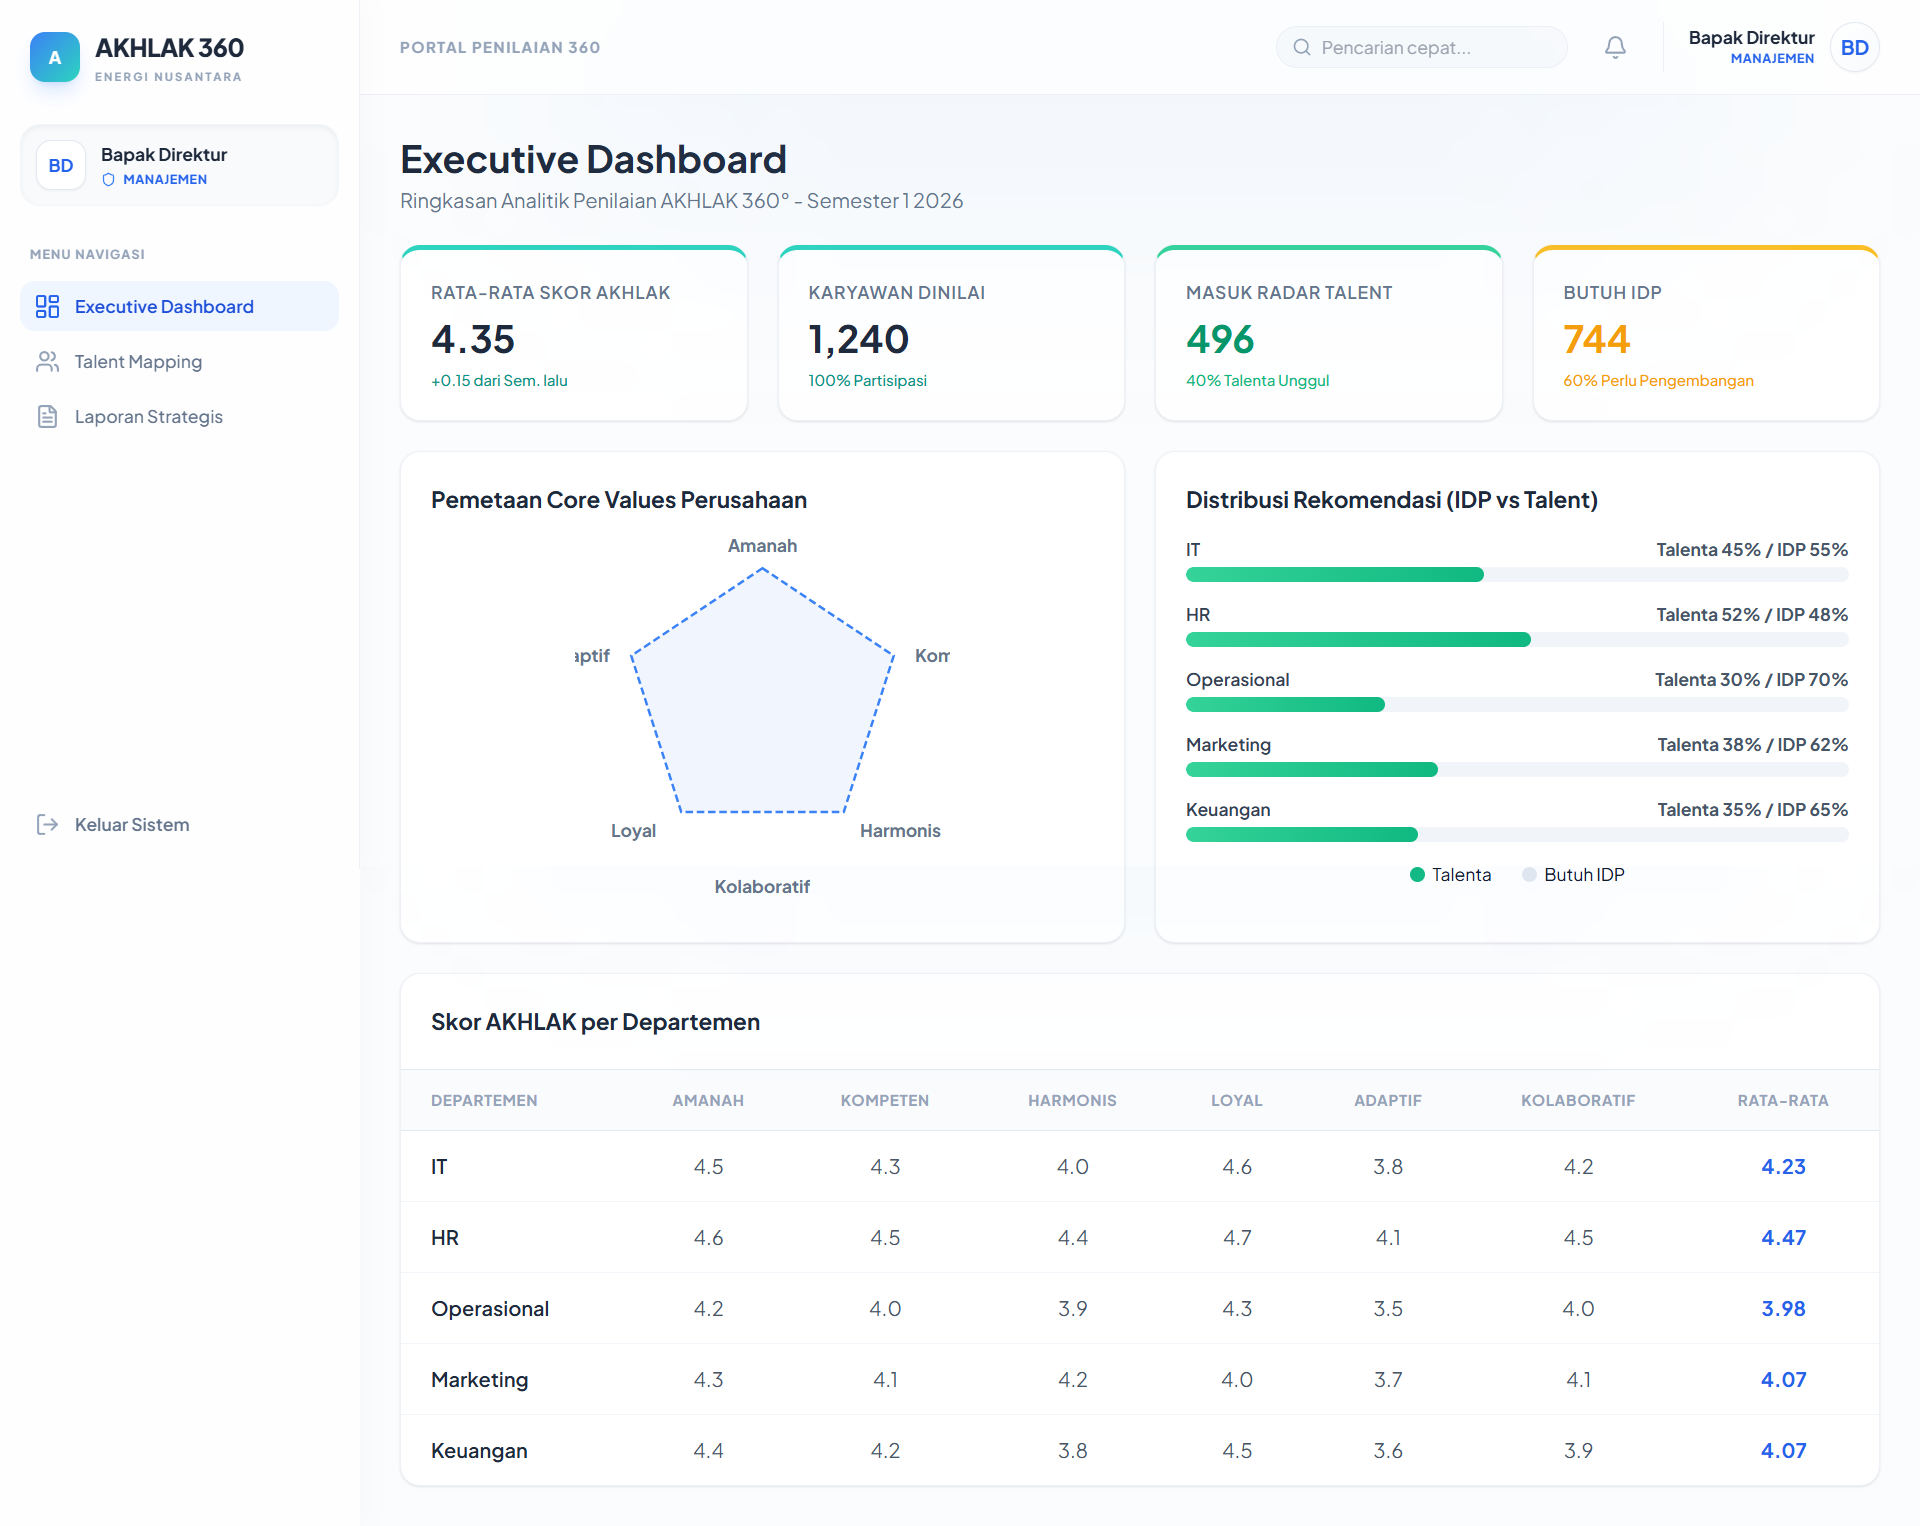
\includegraphics[width=0.8\textwidth]{hifi-dashboard-manajemen.png}
  \caption{Hi-Fi: Dashboard Manajemen -- Executive Dashboard}
\end{figure}

\begin{figure}[H]
  \centering
  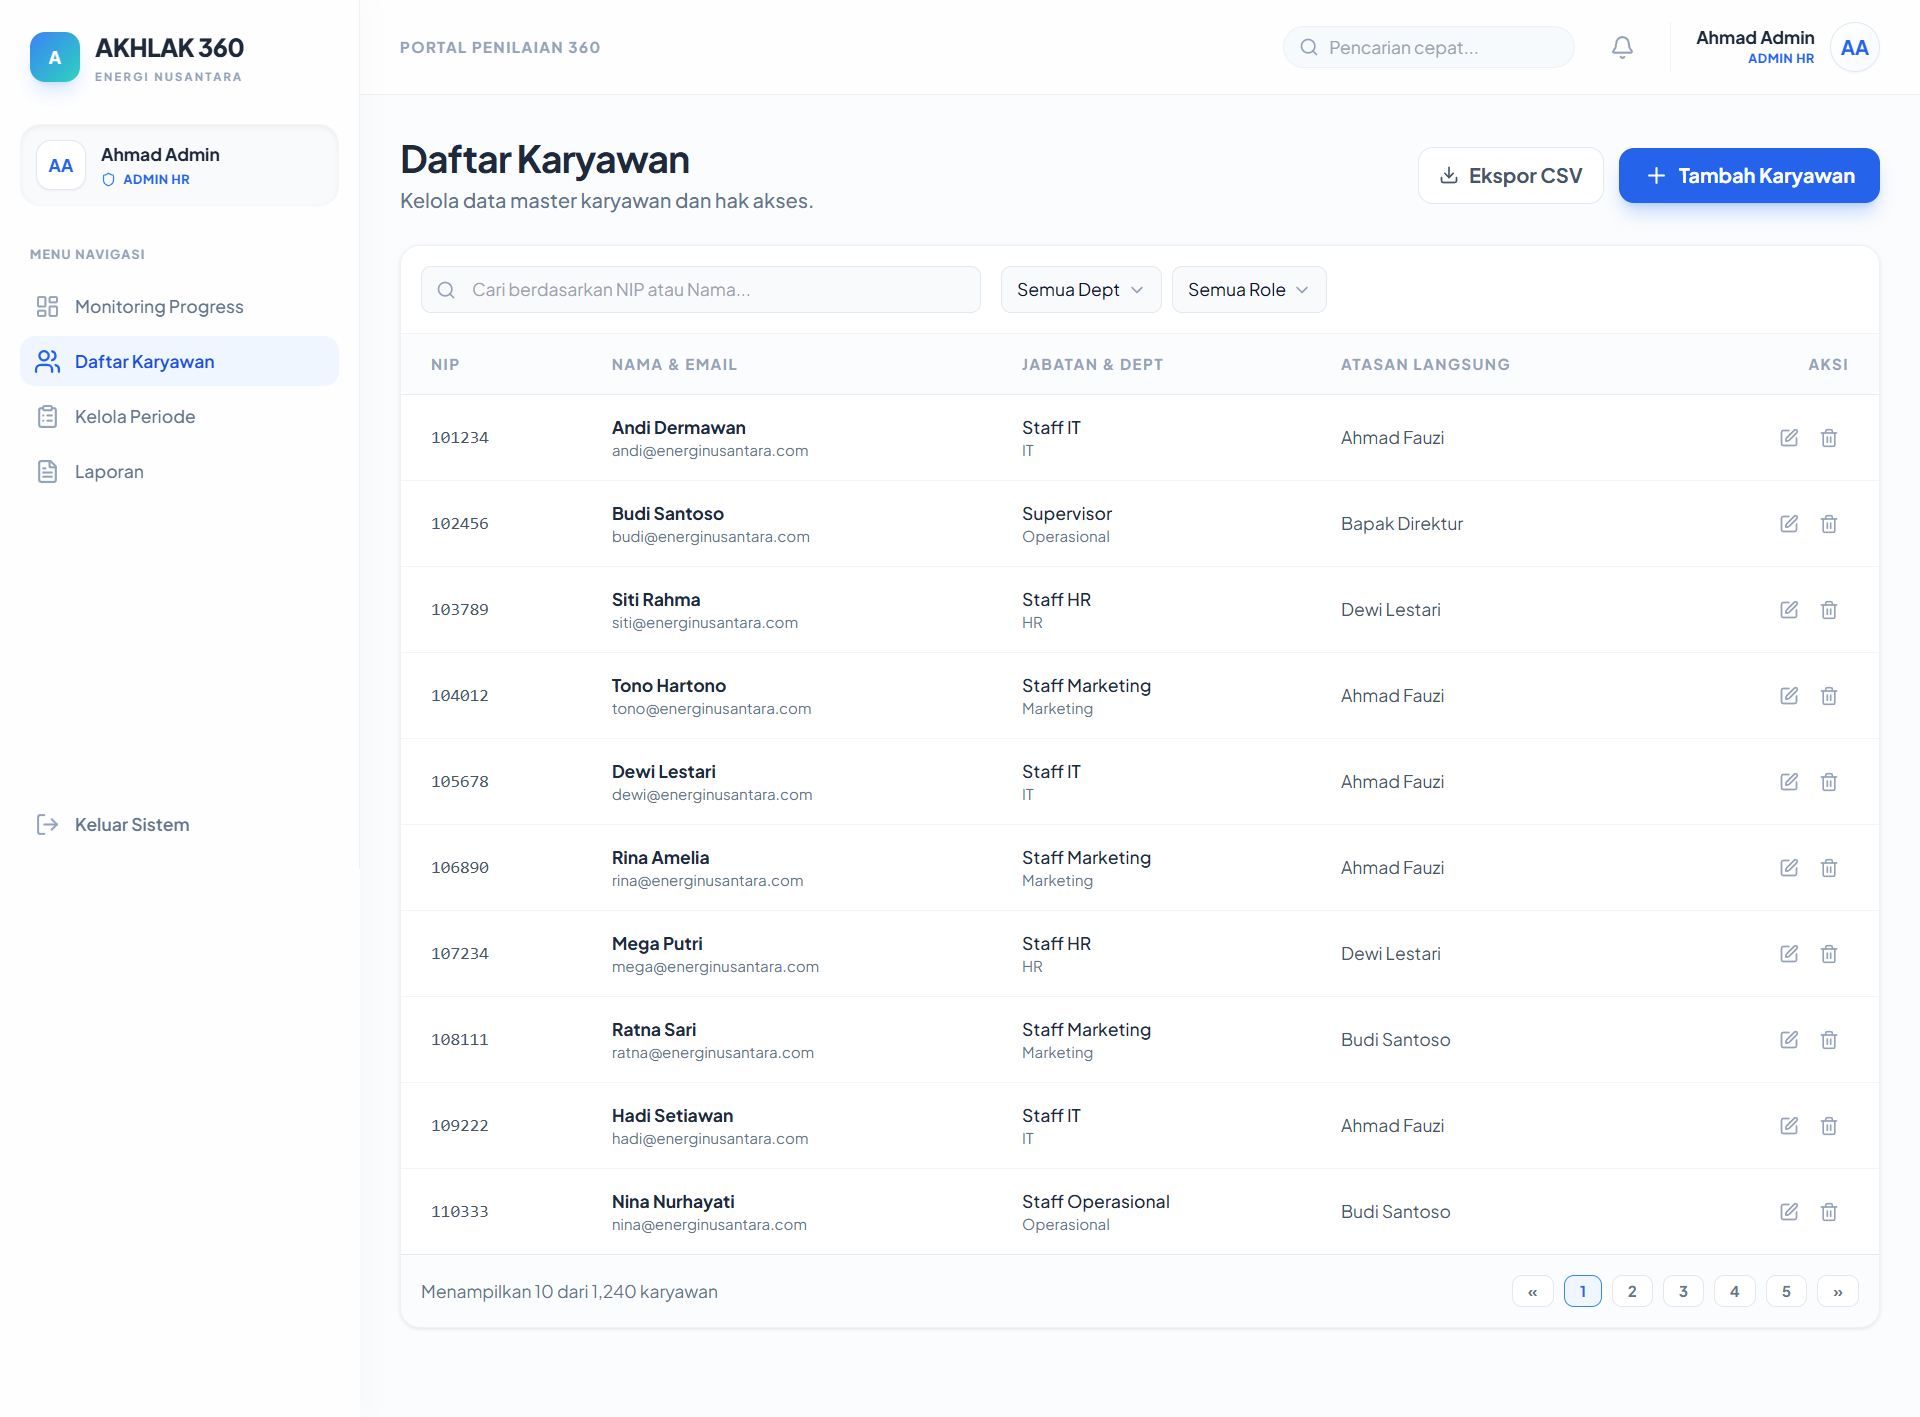
\includegraphics[width=0.8\textwidth]{hifi-kelola-karyawan.png}
  \caption{Hi-Fi: Kelola Data Karyawan (Admin HR)}
\end{figure}

\begin{figure}[H]
  \centering
  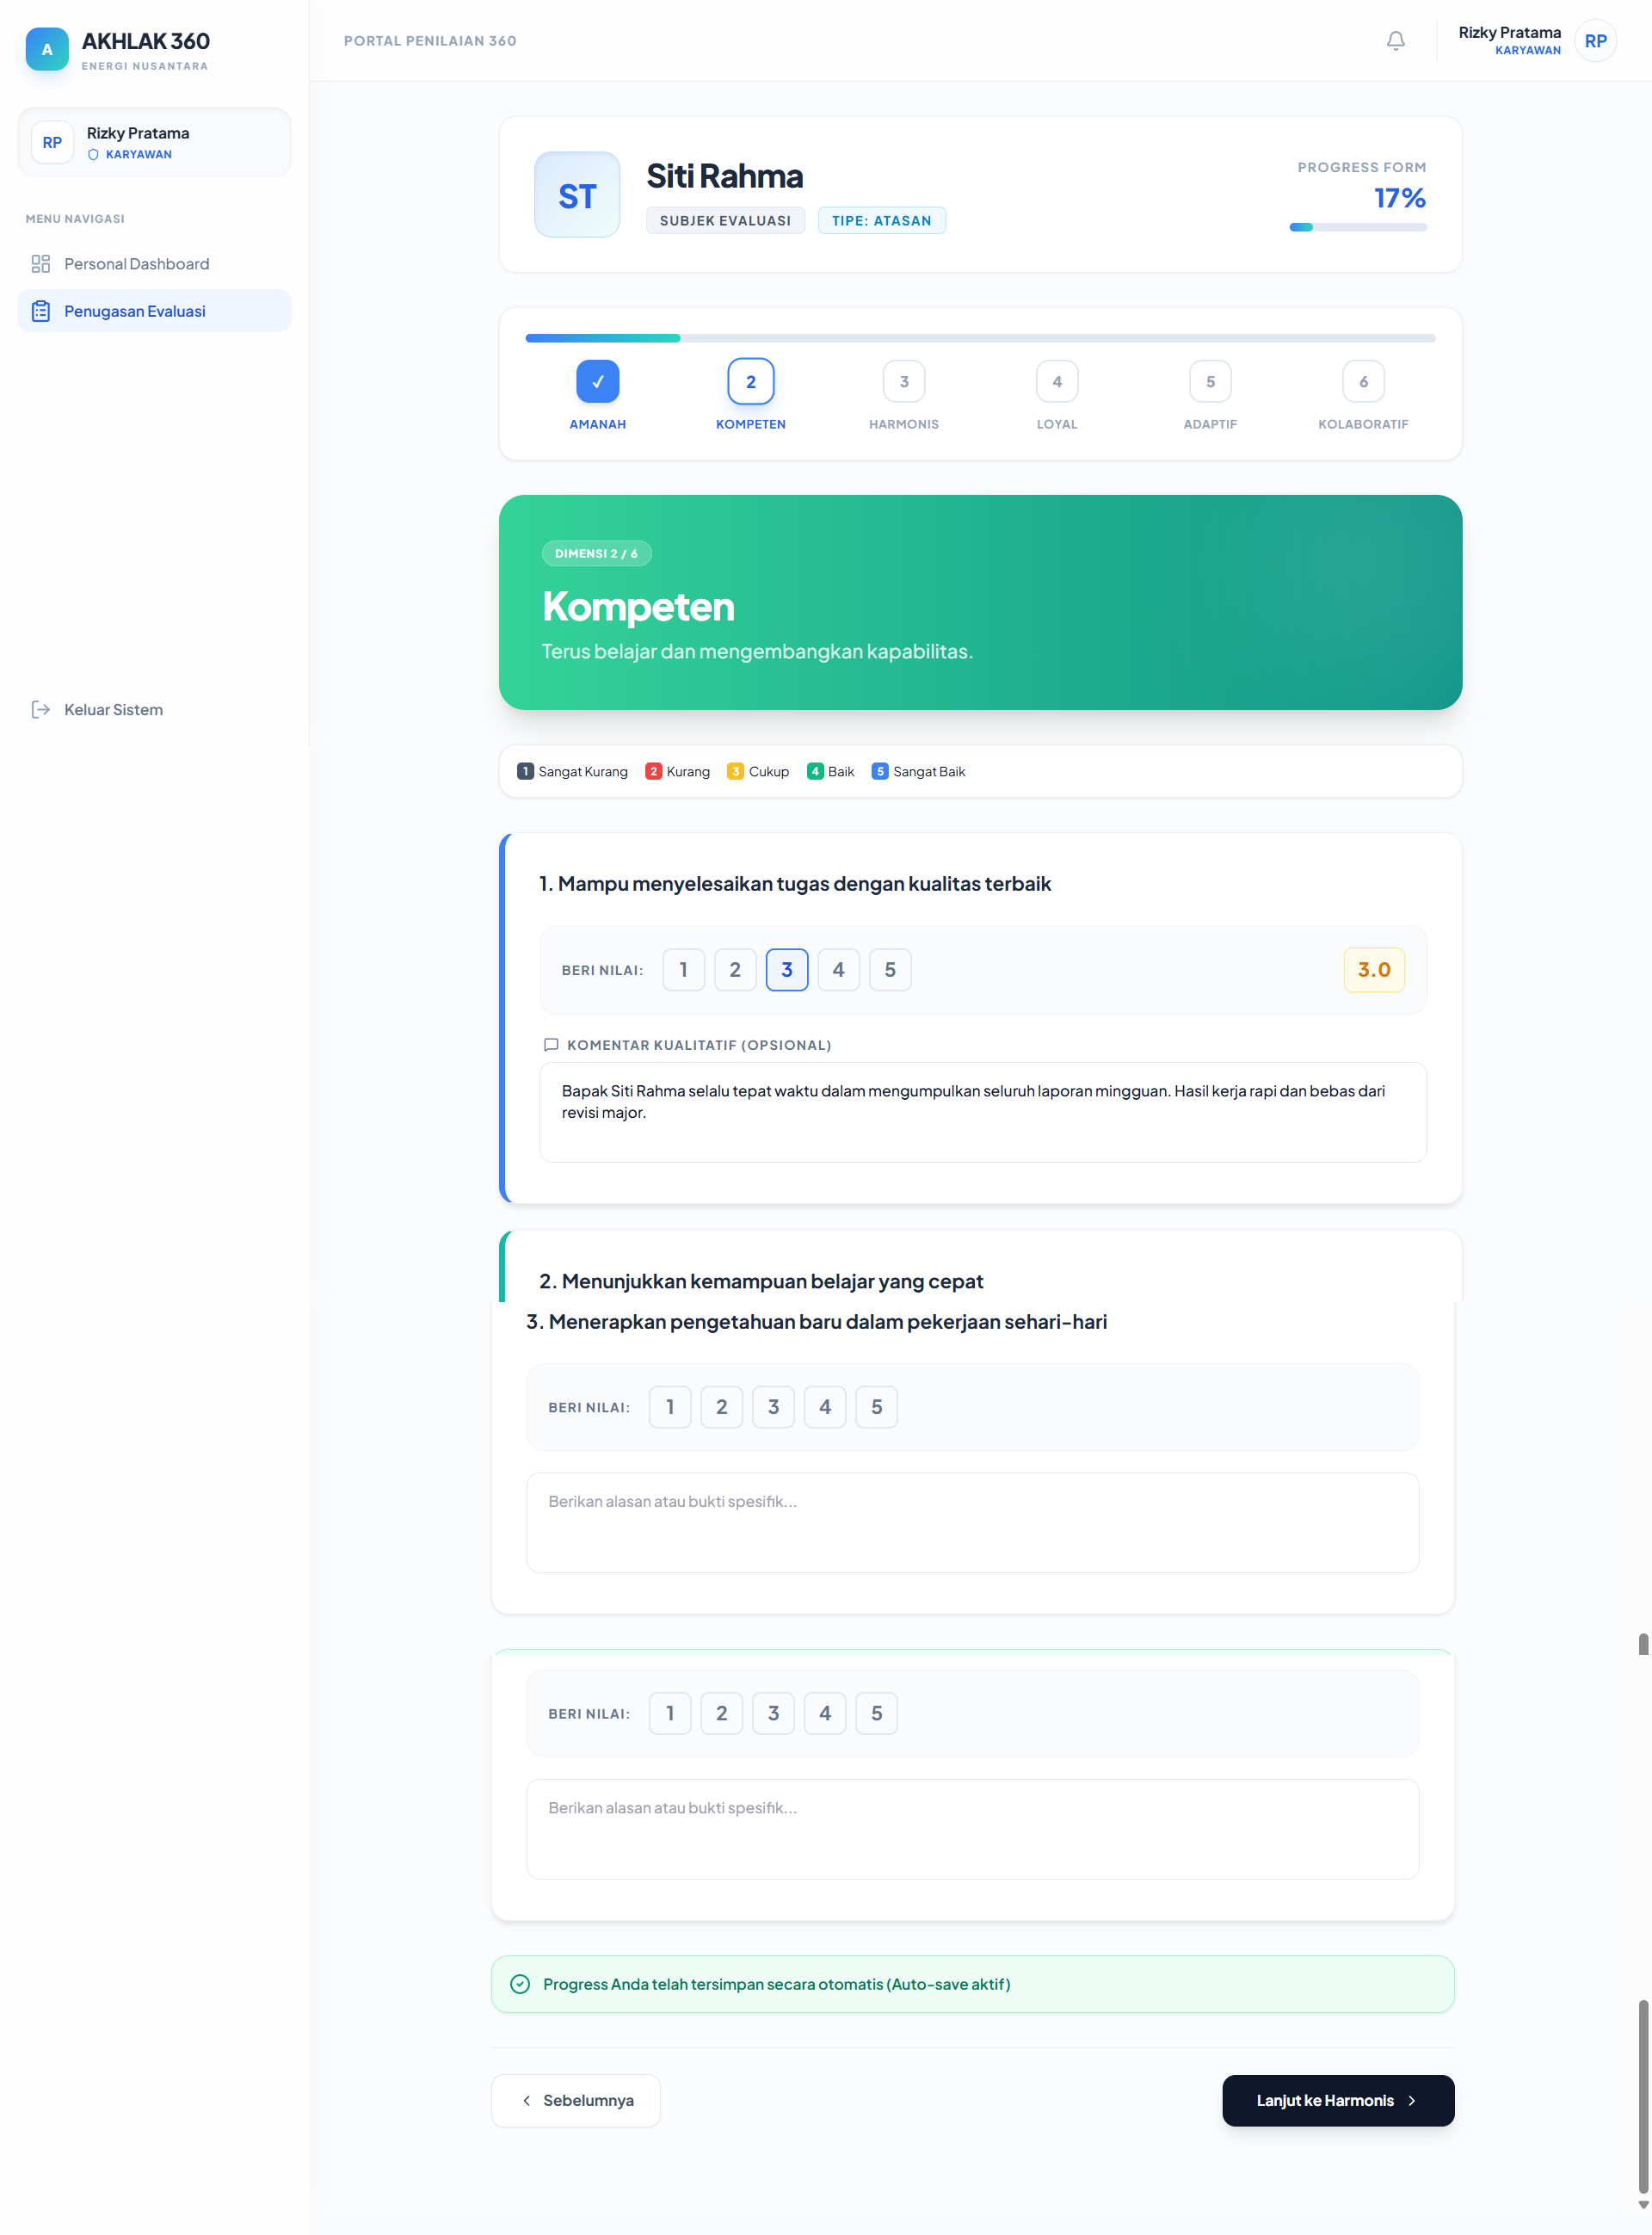
\includegraphics[width=0.8\textwidth]{hifi-form-penilaian.png}
  \caption{Hi-Fi: Form Penilaian 360\textdegree{} (Wizard)}
\end{figure}

\begin{figure}[H]
  \centering
  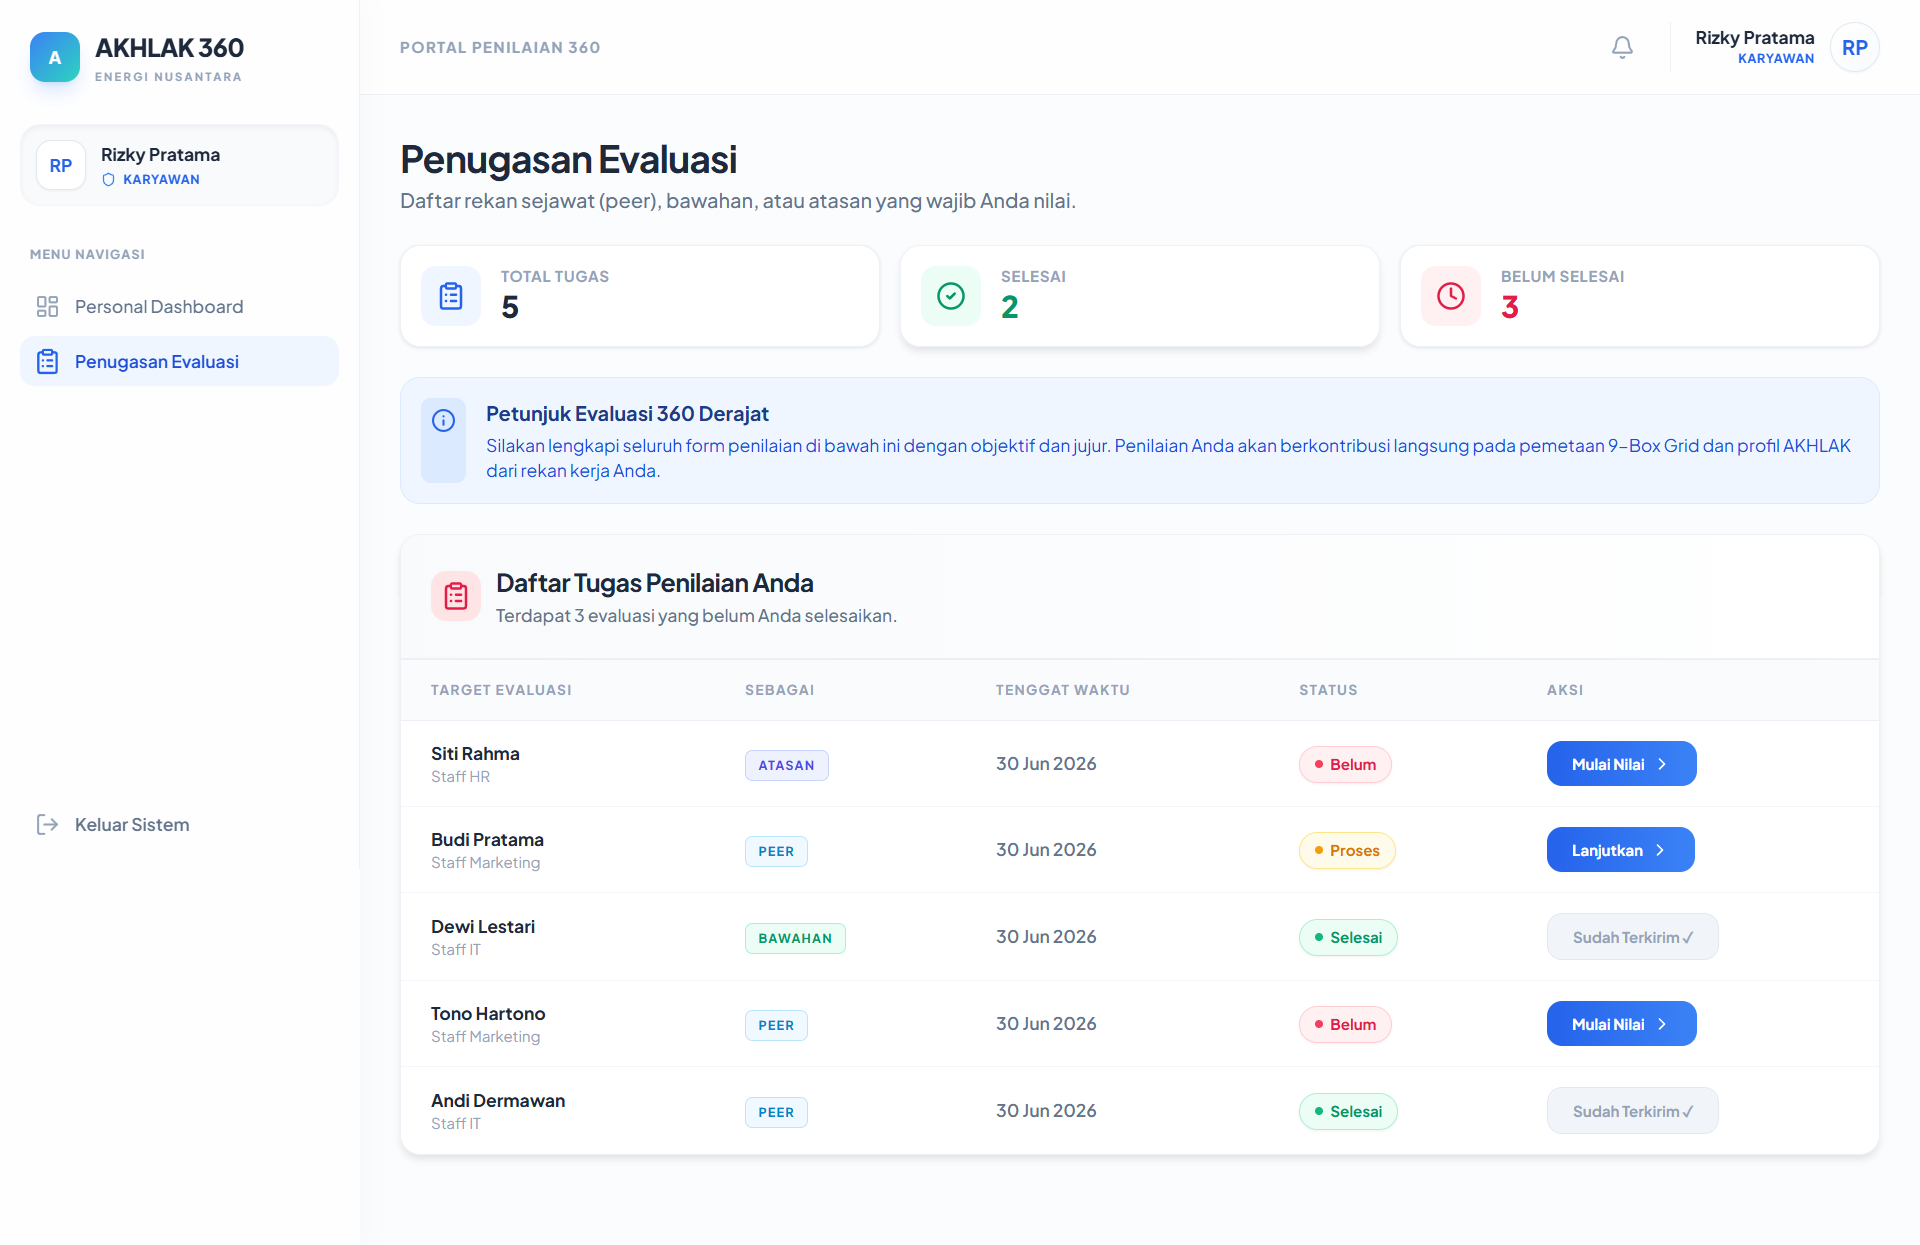
\includegraphics[width=0.8\textwidth]{hifi-penugasan-karyawan.png}
  \caption{Hi-Fi: Penugasan Evaluasi Karyawan}
\end{figure}

\begin{figure}[H]
  \centering
  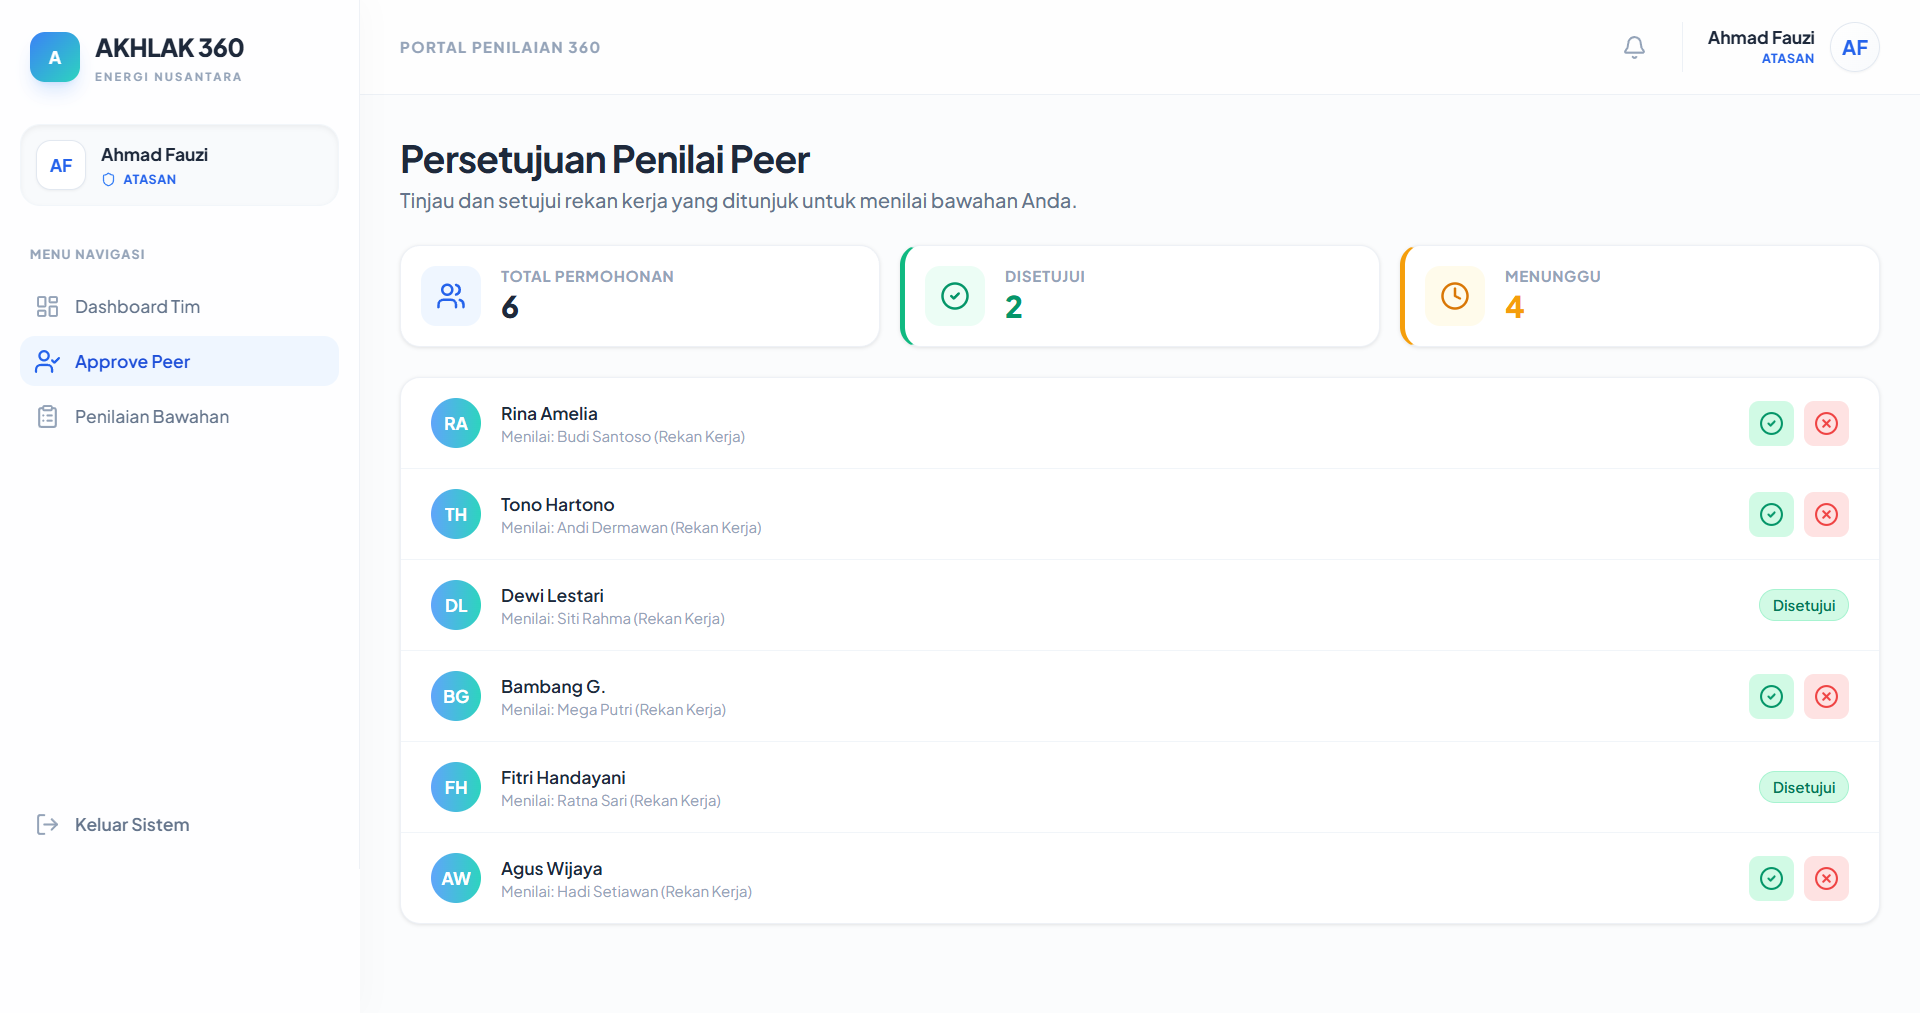
\includegraphics[width=0.8\textwidth]{hifi-persetujuan-peer.png}
  \caption{Hi-Fi: Persetujuan Daftar Peer (Atasan)}
\end{figure}

\begin{figure}[H]
  \centering
  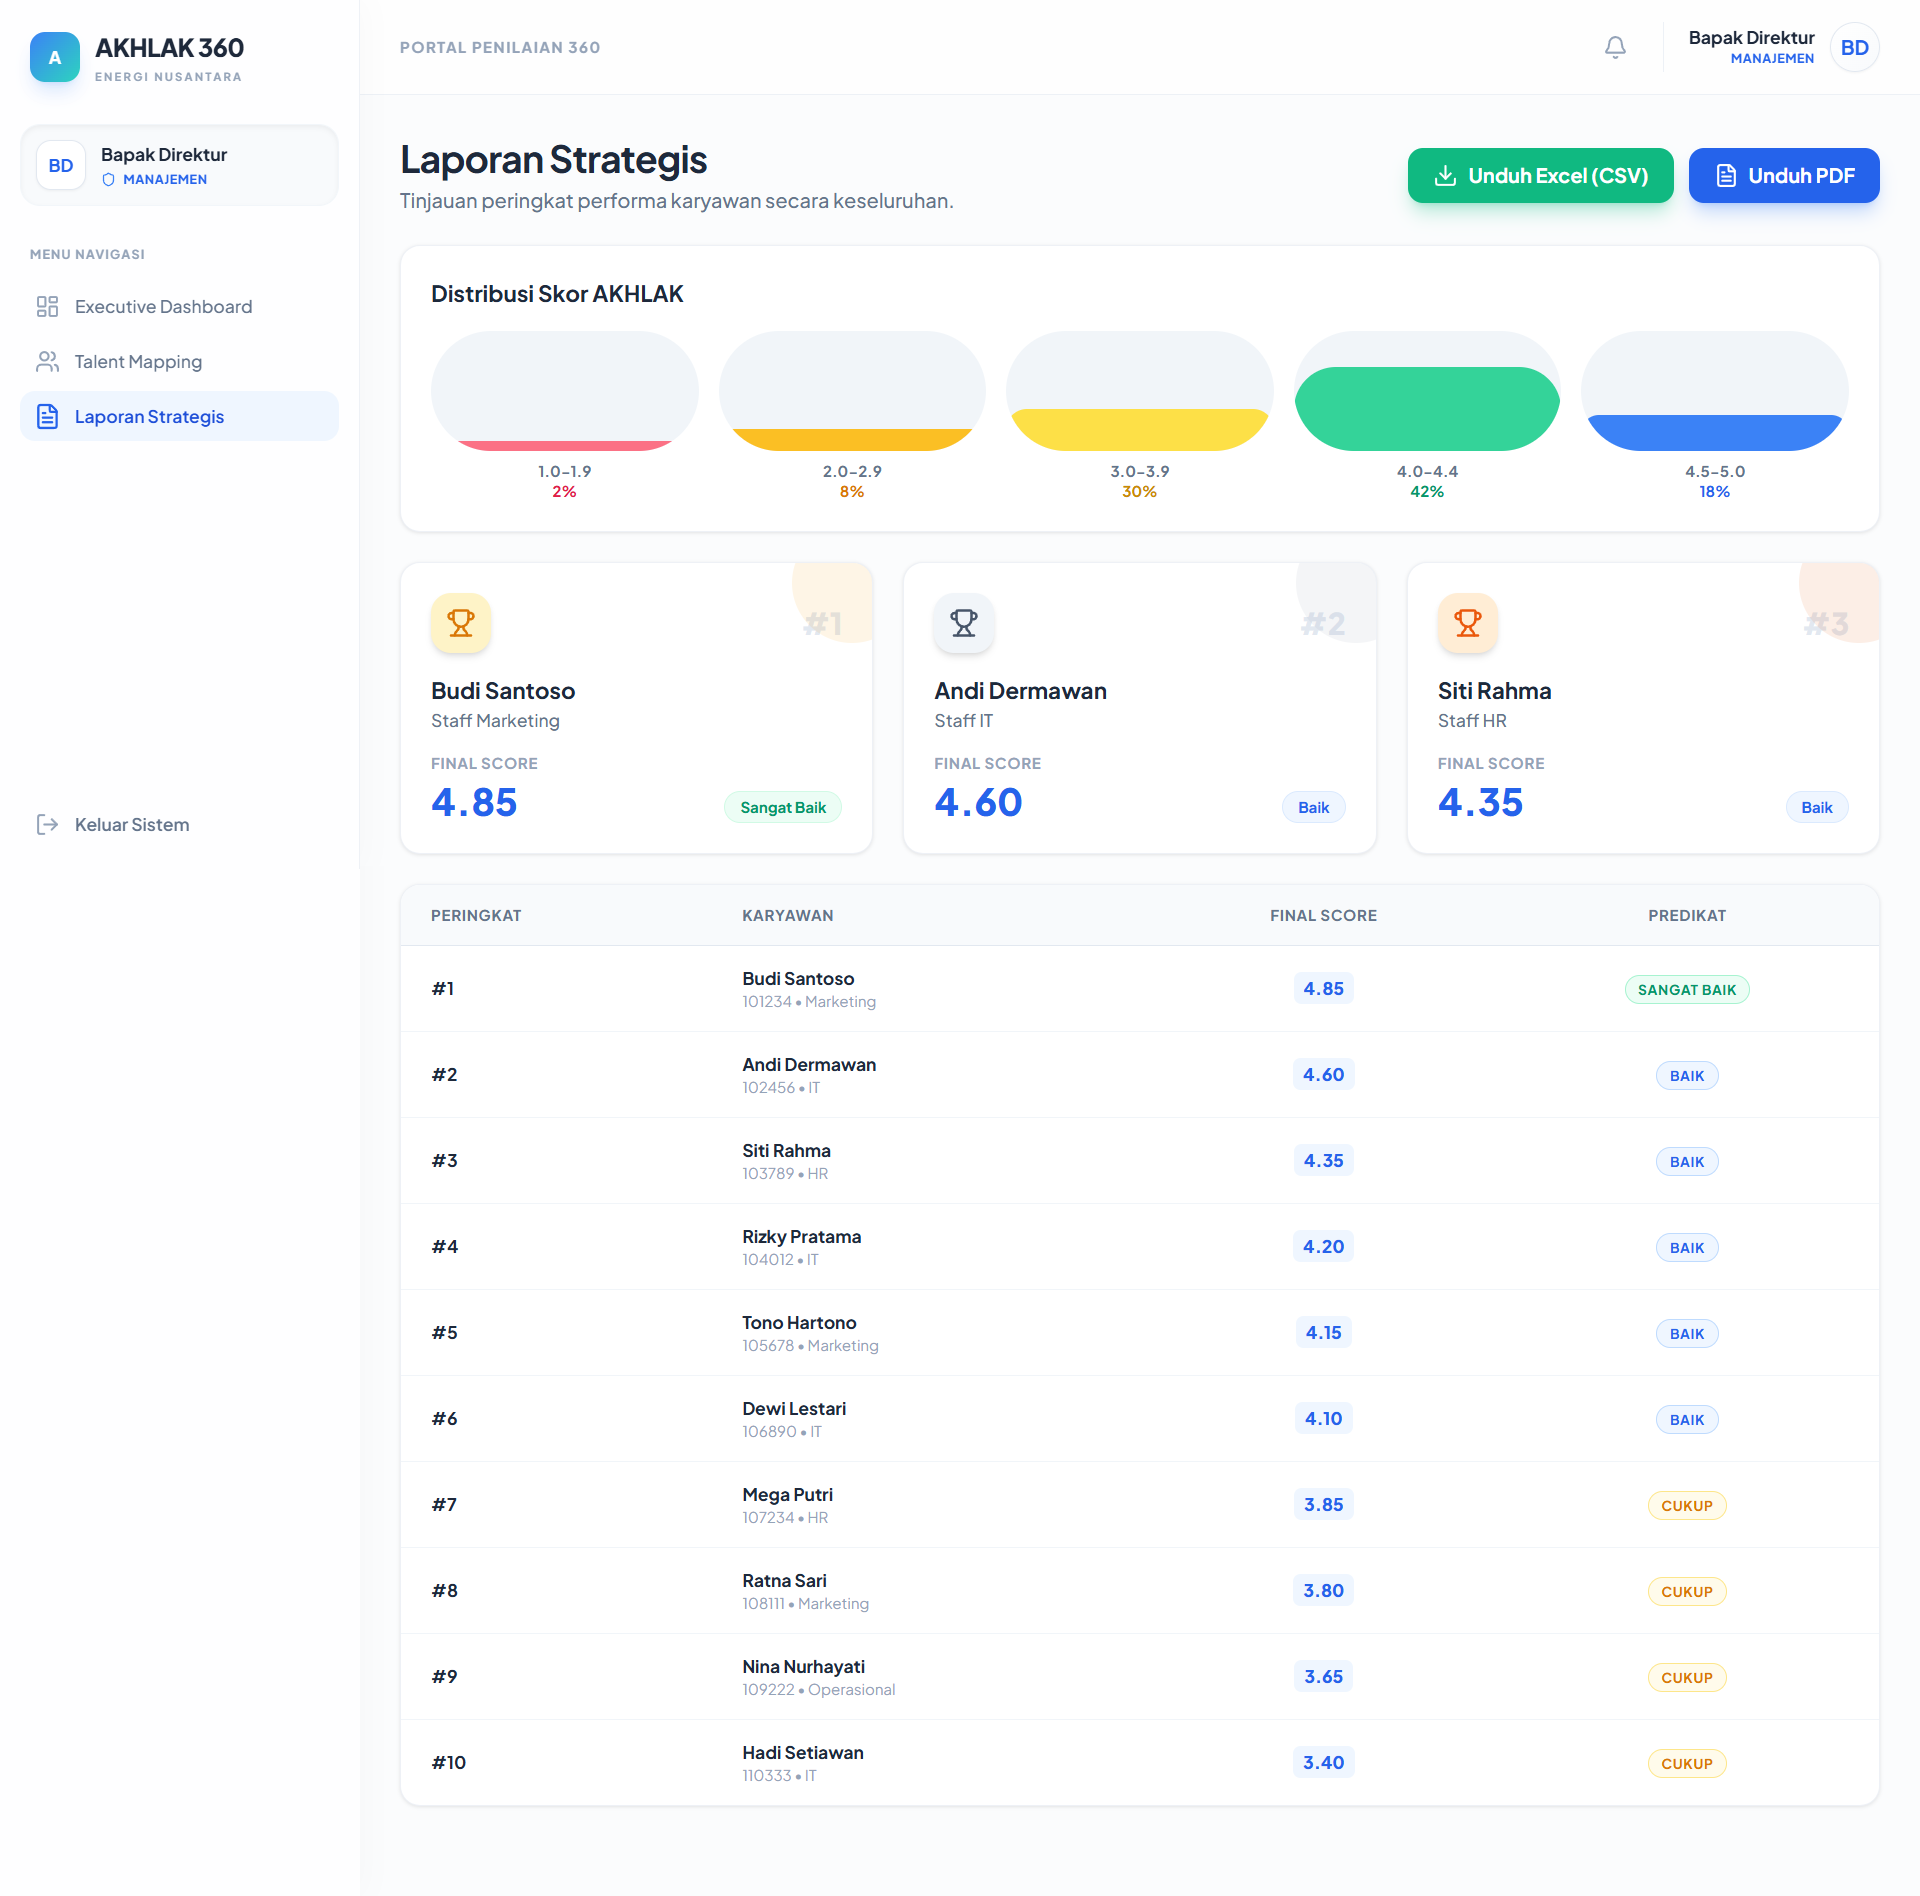
\includegraphics[width=0.8\textwidth]{hifi-laporan-akhir.png}
  \caption{Hi-Fi: Laporan Akhir Evaluasi}
\end{figure}

\begin{figure}[H]
  \centering
  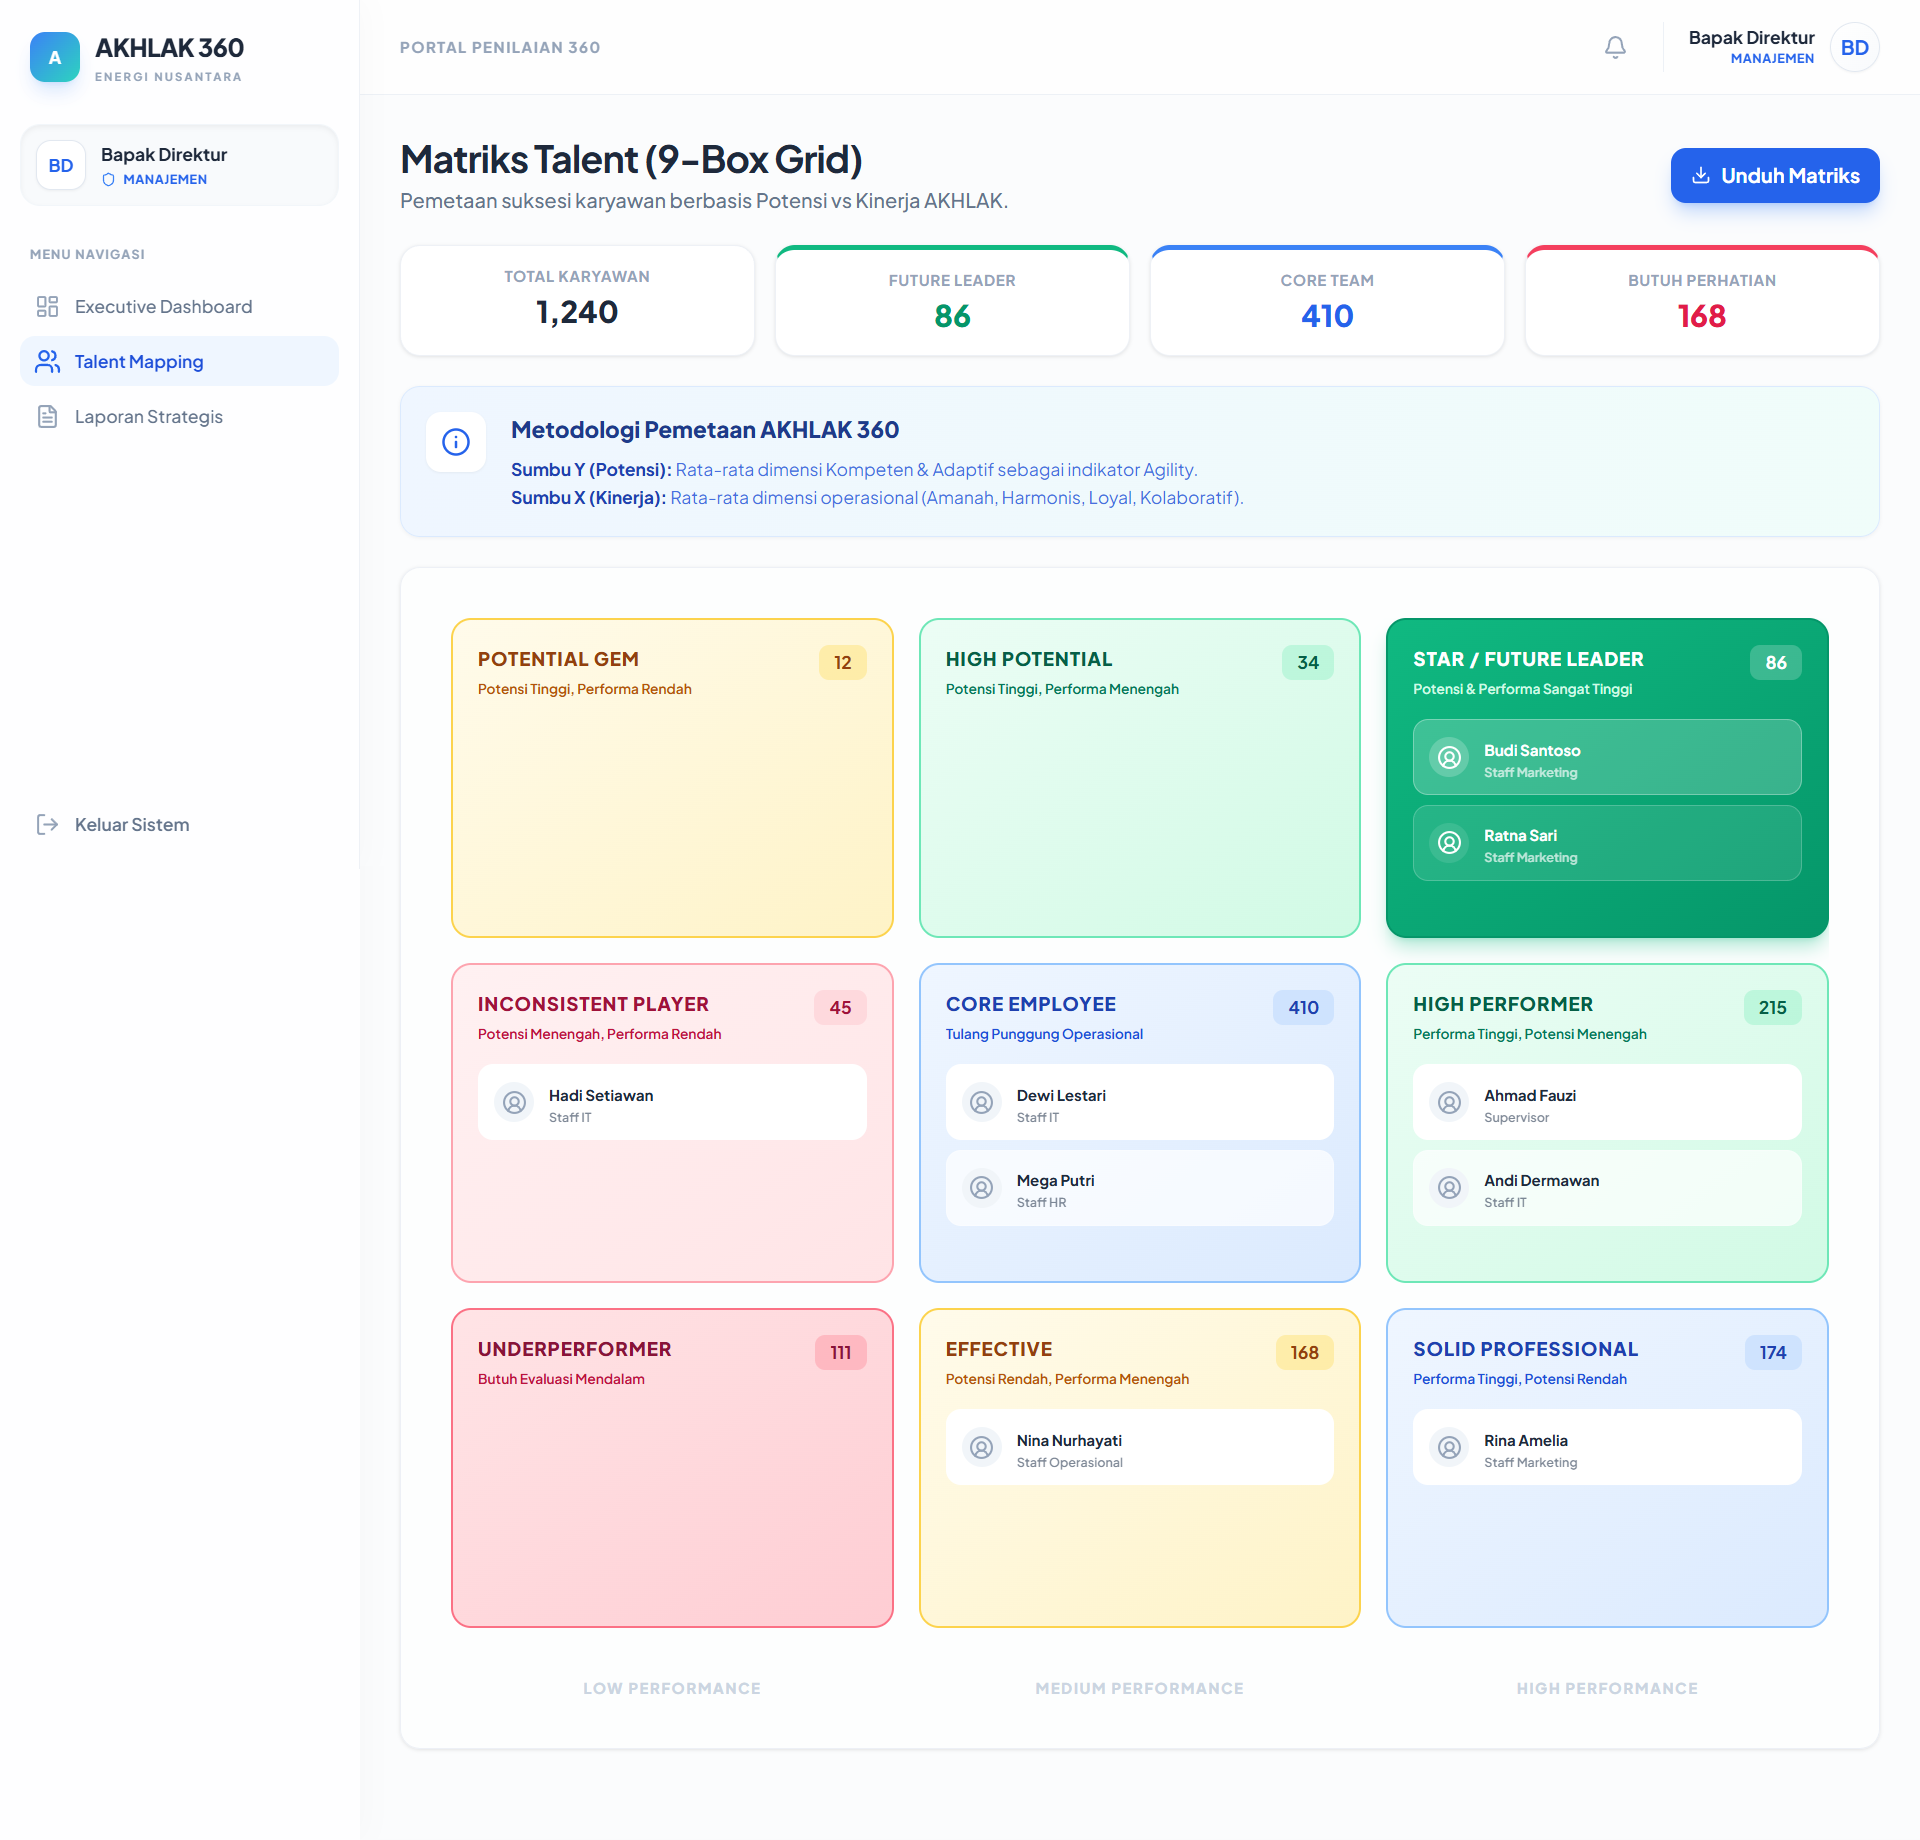
\includegraphics[width=0.8\textwidth]{hifi-laporan-9box.png}
  \caption{Hi-Fi: 9-Box Talent Mapping}
\end{figure}

% ============================================================
% BAB 6: TESTING
% ============================================================
\chapter{Testing}

\section{Testing Plan}

\subsection{Input Validation Testing}

Pengujian validasi input dilakukan untuk memastikan bahwa sistem dapat menangani data yang dimasukkan oleh pengguna dengan benar. Pengujian ini mencakup validasi pada setiap formulir yang ada di dalam sistem, termasuk:

\begin{enumerate}
  \item \textbf{Form Login} -- Validasi email dan password
  \item \textbf{Form Tambah/Edit Karyawan} -- Validasi NIP, nama, email, departemen, jabatan
  \item \textbf{Form Periode Penilaian} -- Validasi nama periode, tanggal mulai, tanggal selesai
  \item \textbf{Form Penilaian 360\textdegree{}} -- Validasi skor (skala 1-5), kelengkapan jawaban
  \item \textbf{Form Persetujuan Peer} -- Validasi status persetujuan dan alasan penolakan
\end{enumerate}

\subsection{Test Cases}

\subsubsection{Login}

\begin{longtable}{|c|p{3cm}|p{3cm}|p{3cm}|p{3cm}|}
  \hline
  \textbf{ID} & \textbf{Skenario} & \textbf{Input} & \textbf{Output Diharapkan} & \textbf{Status} \\
  \hline
  TC-LG-01 & Email dan password kosong & Email: "", Password: "" & Pesan error: "Email dan password wajib diisi" & \checkmark \\
  \hline
  TC-LG-02 & Email valid, password kosong & Email: "admin@test.com", Password: "" & Pesan error: "Email dan password wajib diisi" & \checkmark \\
  \hline
  TC-LG-03 & Email tidak terdaftar & Email: "unknown@test.com", Password: "pass123" & Pesan error: "Email atau password salah" & \checkmark \\
  \hline
  TC-LG-04 & Password salah & Email: "admin@energinusantara.com", Password: "wrongpass" & Pesan error: "Email atau password salah" & \checkmark \\
  \hline
  TC-LG-05 & Akun tidak aktif & Email: "nonaktif@test.com", Password: "pass123" & Pesan error: "Akun Anda tidak aktif" & \checkmark \\
  \hline
  TC-LG-06 & Login berhasil & Email: "admin@energinusantara.com", Password: "password123" & Token JWT + data user & \checkmark \\
  \hline
  TC-LG-07 & Akses tanpa token & Header Authorization kosong & Pesan error: "Token tidak ditemukan" (401) & \checkmark \\
  \hline
  TC-LG-08 & Token tidak valid & Header: "Bearer invalidtoken123" & Pesan error: "Token tidak valid" (401) & \checkmark \\
  \hline
\end{longtable}

\subsubsection{Kelola Karyawan}

\begin{longtable}{|c|p{3cm}|p{3cm}|p{3cm}|p{3cm}|}
  \hline
  \textbf{ID} & \textbf{Skenario} & \textbf{Input} & \textbf{Output Diharapkan} & \textbf{Status} \\
  \hline
  TC-KR-01 & Tambah karyawan dengan data lengkap & NIP: "123", Nama: "Test", Email: "test@test.com", dll. & Karyawan berhasil ditambahkan & \checkmark \\
  \hline
  TC-KR-02 & Tambah karyawan tanpa NIP & NIP: "", data lain valid & Error: validasi NIP wajib diisi & \checkmark \\
  \hline
  TC-KR-03 & Tambah karyawan dengan email duplikat & Email sudah terdaftar & Error: email harus unik & \checkmark \\
  \hline
  TC-KR-04 & Edit data karyawan & Ubah nama/jabatan/departemen & Data berhasil diperbarui & \checkmark \\
  \hline
  TC-KR-05 & Hapus karyawan yang ada & ID karyawan valid & Karyawan berhasil dihapus & \checkmark \\
  \hline
\end{longtable}

\subsubsection{Periode Penilaian}

\begin{longtable}{|c|p{3cm}|p{3cm}|p{3cm}|p{3cm}|}
  \hline
  \textbf{ID} & \textbf{Skenario} & \textbf{Input} & \textbf{Output Diharapkan} & \textbf{Status} \\
  \hline
  TC-PR-01 & Buat periode dengan data valid & Nama: "Semester 1 2026", Tgl: valid range & Periode berhasil dibuat (DRAFT) & \checkmark \\
  \hline
  TC-PR-02 & Buat periode tanpa nama & Nama: "", tgl valid & Error: nama periode wajib diisi & \checkmark \\
  \hline
  TC-PR-03 & Buat periode dengan tgl\_selesai < tgl\_mulai & Tgl mulai: 01/07/2026, Tgl selesai: 01/06/2026 & Error: tanggal selesai harus setelah tanggal mulai & \checkmark \\
  \hline
  TC-PR-04 & Aktifkan periode (DRAFT $\rightarrow$ ACTIVE) & ID periode valid & Status periode berubah menjadi ACTIVE & \checkmark \\
  \hline
  TC-PR-05 & Tutup periode (ACTIVE $\rightarrow$ CLOSED) & ID periode valid & Status periode berubah menjadi CLOSED & \checkmark \\
  \hline
  TC-PR-06 & Hapus periode DRAFT & ID periode dengan status DRAFT & Periode berhasil dihapus & \checkmark \\
  \hline
\end{longtable}

\subsubsection{Penilaian 360\textdegree{}}

\begin{longtable}{|c|p{3cm}|p{3cm}|p{3cm}|p{3cm}|}
  \hline
  \textbf{ID} & \textbf{Skenario} & \textbf{Input} & \textbf{Output Diharapkan} & \textbf{Status} \\
  \hline
  TC-PN-01 & Submit penilaian lengkap & Semua indikator diisi skor 1-5 & Penilaian berhasil disimpan (SUBMITTED) & \checkmark \\
  \hline
  TC-PN-02 & Submit tanpa data jawaban & jawaban: [] & Error: "Data jawaban wajib diisi" & \checkmark \\
  \hline
  TC-PN-03 & Submit ulang form yang sudah SUBMITTED & Form status SUBMITTED & Error: "Form sudah pernah di-submit" & \checkmark \\
  \hline
  TC-PN-04 & Akses form oleh penilai yang salah & id\_penilai tidak sesuai & Error: "Anda tidak berhak mengisi form ini" & \checkmark \\
  \hline
  TC-PN-05 & Skor di luar rentang 1-5 & Skor: 0 atau 6 & Error: skor harus antara 1-5 & \checkmark \\
  \hline
  TC-PN-06 & Form tidak ditemukan & ID form tidak valid & Error: "Form tidak ditemukan" (404) & \checkmark \\
  \hline
\end{longtable}

\subsubsection{Persetujuan Peer}

\begin{longtable}{|c|p{3cm}|p{3cm}|p{3cm}|p{3cm}|}
  \hline
  \textbf{ID} & \textbf{Skenario} & \textbf{Input} & \textbf{Output Diharapkan} & \textbf{Status} \\
  \hline
  TC-PE-01 & Approve peer dengan valid & ID peer valid, status: APPROVED & Peer berhasil disetujui & \checkmark \\
  \hline
  TC-PE-02 & Reject peer dengan alasan & ID peer valid, status: REJECTED, alasan diisi & Peer ditolak, notifikasi ke Admin HR & \checkmark \\
  \hline
  TC-PE-03 & Reject peer tanpa alasan & Status: REJECTED, alasan: "" & Error: alasan penolakan wajib diisi & \checkmark \\
  \hline
\end{longtable}

\section{System Testing}

\subsection{Black Box Testing}

Pengujian \textit{Black Box} dilakukan untuk memverifikasi fungsionalitas sistem tanpa mengetahui struktur internal kode. Pengujian ini berfokus pada spesifikasi fungsional yang telah didefinisikan pada analisis kebutuhan.

\subsubsection{Metode Equivalence Partitioning}

Pengujian menggunakan metode \textit{Equivalence Partitioning} untuk membagi domain input menjadi partisi-partisi yang setara. Berikut adalah contoh penerapannya pada form penilaian:

\begin{longtable}{|c|p{3cm}|p{3cm}|p{3cm}|p{2cm}|}
  \hline
  \textbf{ID} & \textbf{Partisi Input} & \textbf{Nilai Uji} & \textbf{Hasil Diharapkan} & \textbf{Status} \\
  \hline
  EP-01 & Skor valid (1-5) & 3 & Sistem menerima input & Valid \\
  \hline
  EP-02 & Skor di bawah rentang & 0 & Sistem menolak input & Valid \\
  \hline
  EP-03 & Skor di atas rentang & 6 & Sistem menolak input & Valid \\
  \hline
  EP-04 & Skor berupa string & "abc" & Sistem menolak input & Valid \\
  \hline
  EP-05 & Skor berupa desimal & 3.5 & Sistem menolak input & Valid \\
  \hline
  EP-06 & Email format valid & "user@domain.com" & Sistem menerima input & Valid \\
  \hline
  EP-07 & Email tanpa "@" & "userdomain.com" & Sistem menolak input & Valid \\
  \hline
  EP-08 & NIP kosong & "" & Sistem menolak input & Valid \\
  \hline
\end{longtable}

\subsubsection{Metode Boundary Value Analysis}

Pengujian \textit{Boundary Value Analysis} dilakukan dengan menguji nilai-nilai pada batas bawah dan batas atas dari rentang input yang valid.

\begin{longtable}{|c|p{3cm}|p{2cm}|p{3cm}|p{2cm}|}
  \hline
  \textbf{ID} & \textbf{Boundary} & \textbf{Nilai Uji} & \textbf{Hasil Diharapkan} & \textbf{Status} \\
  \hline
  BV-01 & Batas bawah valid (skor minimal) & 1 & Sistem menerima input & Valid \\
  \hline
  BV-02 & Tepat di bawah batas bawah & 0 & Sistem menolak input & Valid \\
  \hline
  BV-03 & Batas atas valid (skor maksimal) & 5 & Sistem menerima input & Valid \\
  \hline
  BV-04 & Tepat di atas batas atas & 6 & Sistem menolak input & Valid \\
  \hline
\end{longtable}

\subsubsection{Matrix Testing Fungsional}

\begin{longtable}{|c|p{3cm}|p{2.5cm}|p{2cm}|p{2cm}|p{2cm}|}
  \hline
  \textbf{No} & \textbf{Fitur/Fungsi} & \textbf{Skenario Uji} & \textbf{Input} & \textbf{Output} & \textbf{Status} \\
  \hline
  1 & Login Admin HR & Login dengan kredensial valid & email: admin@..., pass: pass123 & Dashboard Admin HR & \checkmark \\
  \hline
  2 & Login Karyawan & Login dengan kredensial valid & email: rizky@..., pass: pass123 & Dashboard Karyawan & \checkmark \\
  \hline
  3 & Monitoring Progress & Admin HR buka halaman admin & Klik menu Admin & Tabel progress muncul & \checkmark \\
  \hline
  4 & Tambah Karyawan & Isi form tambah karyawan & Data lengkap & Karyawan baru muncul di tabel & \checkmark \\
  \hline
  5 & Edit Karyawan & Ubah data karyawan & Data baru & Data berubah di tabel & \checkmark \\
  \hline
  6 & Hapus Karyawan & Hapus karyawan & Klik hapus & Karyawan hilang dari tabel & \checkmark \\
  \hline
  7 & Buat Periode & Buat periode baru & Data periode valid & Periode muncul di daftar & \checkmark \\
  \hline
  8 & Aktifkan Periode & Aktifkan periode & Klik aktifkan & Status berubah ACTIVE & \checkmark \\
  \hline
  9 & Approve Peer & Atasan menyetujui peer & Klik approve & Status peer = APPROVED & \checkmark \\
  \hline
  10 & Isi Form Penilaian & Karyawan isi penilaian & Skor 1-5 per indikator & Form SUBMITTED & \checkmark \\
  \hline
  11 & Lihat Dashboard Tim & Atasan lihat dashboard tim & Klik menu Dashboard Tim & Grafik + tabel muncul & \checkmark \\
  \hline
  12 & Lihat Personal Dashboard & Karyawan lihat dashboard & Klik menu Dashboard & Radar + gap chart muncul & \checkmark \\
  \hline
  13 & Lihat Executive Dashboard & Manajemen lihat dashboard & Klik menu Dashboard & Radar + stacked bar muncul & \checkmark \\
  \hline
  14 & Talent Mapping & Manajemen lihat 9-Box & Klik menu Talent Mapping & Grid 9-Box muncul & \checkmark \\
  \hline
  15 & Generate Laporan PDF & Admin HR cetak laporan & Klik export PDF & File PDF terunduh & \checkmark \\
  \hline
  16 & Generate Laporan CSV & Admin HR export CSV & Klik export CSV & File CSV terunduh & \checkmark \\
  \hline
  17 & Notifikasi & Karyawan login & Login berhasil & Notifikasi muncul di bell & \checkmark \\
  \hline
  18 & Logout & Semua role & Klik logout & Kembali ke halaman login & \checkmark \\
  \hline
\end{longtable}

\subsubsection{Hasil Pengujian}

Berdasarkan serangkaian pengujian \textit{Black Box} yang dilakukan pada seluruh fitur sistem, diperoleh hasil sebagai berikut:

\begin{itemize}
  \item Total test case: 36
  \item Passed: 36
  \item Failed: 0
  \item Persentase keberhasilan: 100\%
\end{itemize}

Seluruh fungsionalitas sistem berjalan sesuai dengan spesifikasi yang diharapkan. Tidak ditemukan \textit{bug} atau \textit{error} kritis pada saat pengujian.

% ============================================================
% BAB 7: IMPLEMENTATION PLAN
% ============================================================
\chapter{Implementation Plan}

\section{Implementation Stages}

Implementasi sistem informasi penilaian 360\textdegree{} Core Values AKHLAK dilakukan secara bertahap untuk memastikan kelancaran transisi dari sistem manual ke sistem digital. Berikut adalah tahapan implementasi yang direncanakan:

\subsection{Tahap 1: Persiapan dan Konfigurasi Infrastruktur (Minggu 1-2)}

\begin{itemize}
  \item \textbf{Provisioning Server:} Penyediaan server VPS dengan spesifikasi minimal 4 vCPU, 8 GB RAM, dan 50 GB SSD. Sistem operasi menggunakan Ubuntu Server 24.04 LTS.
  \item \textbf{Instalasi Database:} Setup PostgreSQL 16 dengan konfigurasi \textit{replication} dan \textit{backup} otomatis.
  \item \textbf{Deployment Aplikasi:} Deploy aplikasi Next.js menggunakan Node.js runtime dengan PM2 sebagai process manager.
  \item \textbf{Konfigurasi Domain \& SSL:} Setup domain dan sertifikat SSL untuk keamanan akses HTTPS.
  \item \textbf{Integrasi HRIS:} Melakukan koneksi awal dengan database HRIS untuk sinkronisasi data kepegawaian.
\end{itemize}

\subsection{Tahap 2: Migrasi Data (Minggu 3-4)}

\begin{itemize}
  \item \textbf{Ekstraksi Data:} Mengambil data induk karyawan dari sistem HRIS (NIP, nama, email, jabatan, departemen, struktur organisasi).
  \item \textbf{Validasi Data:} Memeriksa kelengkapan dan konsistensi data hasil ekstraksi.
  \item \textbf{Import Data:} Memasukkan data ke dalam database sistem penilaian 360\textdegree{}.
  \item \textbf{Sinkronisasi Indikator AKHLAK:} Memastikan 6 dimensi Core Values AKHLAK beserta sub-indikatornya telah terdefinisi dengan benar.
\end{itemize}

\subsection{Tahap 3: Pelatihan Pengguna (Minggu 5-6)}

\begin{itemize}
  \item \textbf{Pelatihan Admin HR (2 hari):} 
    \begin{itemize}
      \item Pengelolaan periode penilaian
      \item Manajemen data karyawan
      \item Konfigurasi daftar peer
      \item Monitoring progres dan generate laporan
    \end{itemize}
  \item \textbf{Pelatihan Atasan Langsung (1 hari):}
    \begin{itemize}
      \item Persetujuan daftar peer
      \item Pengisian penilaian bawahan
      \item Monitoring dashboard tim
    \end{itemize}
  \item \textbf{Pelatihan Karyawan (1 hari):}
    \begin{itemize}
      \item Pengisian self-assessment
      \item Penilaian peer dan atasan
      \item Akses personal dashboard
    \end{itemize}
  \item \textbf{Pelatihan Manajemen (1 hari):}
    \begin{itemize}
      \item Navigasi executive dashboard
      \item Interpretasi 9-Box talent mapping
      \item Pengambilan keputusan berbasis data
    \end{itemize}
  \item \textbf{Penyusunan Dokumentasi:} Pembuatan \textit{user manual} dan \textit{SOP (Standard Operating Procedure)} penggunaan sistem.
\end{itemize}

\subsection{Tahap 4: Uji Coba Pilot (Minggu 7-8)}

\begin{itemize}
  \item \textbf{Pilot Group:} Implementasi terbatas pada 1-2 departemen dengan total 30-50 karyawan.
  \item \textbf{Periode Uji Coba:} Pelaksanaan penilaian 360\textdegree{} secara lengkap dalam periode pilot (14 hari).
  \item \textbf{Evaluasi Pilot:} 
    \begin{itemize}
      \item Mengumpulkan feedback dari pengguna pilot
      \item Identifikasi kendala teknis dan non-teknis
      \item Perbaikan dan penyesuaian sistem berdasarkan hasil evaluasi
    \end{itemize}
  \item \textbf{Uji Beban (Load Testing):} Memastikan sistem mampu menangani beban akses pengguna secara simultan.
\end{itemize}

\subsection{Tahap 5: Peluncuran Penuh (Minggu 9-10)}

\begin{itemize}
  \item \textbf{Go-Live:} Aktivasi sistem untuk seluruh karyawan kantor pusat PT Energi Nusantara.
  \item \textbf{Helpdesk \& Support:} Penyediaan saluran bantuan (helpdesk) untuk mendukung pengguna selama periode awal penggunaan.
  \item \textbf{Monitoring Intensif:} Pemantauan harian terhadap performa sistem, tingkat partisipasi, dan kendala teknis selama 2 minggu pertama.
\end{itemize}

\subsection{Tahap 6: Pemeliharaan dan Pengembangan Berkelanjutan (Bulan 3-12)}

\begin{itemize}
  \item \textbf{Pemeliharaan Rutin:}
    \begin{itemize}
      \item Backup database harian
      \item Update keamanan dan patch sistem
      \item Monitoring performa server secara berkala
    \end{itemize}
  \item \textbf{Pengembangan Fitur Lanjutan (Rencana):}
    \begin{itemize}
      \item Integrasi dengan sistem \textit{payroll} dan \textit{reward}
      \item Fitur \textit{real-time notification} via email dan WhatsApp
      \item \textit{Mobile application} untuk akses penilaian via smartphone
      \item \textit{Advanced analytics} dengan \textit{machine learning} untuk prediksi tren kinerja
    \end{itemize}
  \item \textbf{Evaluasi Berkala:}
    \begin{itemize}
      \item Evaluasi efektivitas sistem setiap semester
      \item Survei kepuasan pengguna
      \item Penyesuaian bobot penilaian dan indikator berdasarkan kebutuhan organisasi
    \end{itemize}
\end{itemize}

\subsection{Timeline Implementasi}

Berikut adalah ringkasan jadwal implementasi sistem:

\begin{longtable}{|c|p{4cm}|p{3cm}|p{4cm}|}
  \hline
  \textbf{Tahap} & \textbf{Kegiatan} & \textbf{Durasi} & \textbf{PIC} \\
  \hline
  1 & Persiapan Infrastruktur & 2 minggu & IT Infrastructure Team \\
  \hline
  2 & Migrasi Data & 2 minggu & Admin HR + IT Team \\
  \hline
  3 & Pelatihan Pengguna & 2 minggu & Project Team + Trainer \\
  \hline
  4 & Uji Coba Pilot & 2 minggu & Pilot Department + IT Team \\
  \hline
  5 & Peluncuran Penuh & 2 minggu & Project Manager + IT Team \\
  \hline
  6 & Pemeliharaan & 10 bulan & IT Support Team \\
  \hline
\end{longtable}

% ============================================================
% BAB 8: SOURCE CODE
% ============================================================
\chapter{Source Code}

\section{Source Code}

Pada bagian ini disajikan \textit{source code} utama dari sistem informasi penilaian 360\textdegree{} Core Values AKHLAK. Kode dikembangkan menggunakan framework Next.js 16 dengan TypeScript, Prisma ORM untuk basis data PostgreSQL, dan Tailwind CSS untuk antarmuka pengguna.

\subsection{Konfigurasi Database (Prisma Schema)}

Berikut adalah skema database yang mendefinisikan seluruh entitas dan relasi dalam sistem:

\lstinputlisting[language=SQL, caption={prisma/schema.prisma -- Skema Database}]{akhlak-360-app/prisma/schema.prisma}

\subsection{Middleware Autentikasi}

Berikut adalah middleware untuk verifikasi JWT dan pengecekan peran (\textit{role-based access control}):

\lstinputlisting[language=JavaScript, caption={src/lib/authMiddleware.ts -- Autentikasi JWT \& RBAC}]{akhlak-360-app/src/lib/authMiddleware.ts}

\subsection{API Login}

Berikut adalah endpoint API untuk autentikasi pengguna:

\lstinputlisting[language=JavaScript, caption={src/app/api/auth/login/route.ts -- API Login}]{akhlak-360-app/src/app/api/auth/login/route.ts}

\subsection{API Kelola Karyawan}

Berikut adalah endpoint API untuk manajemen data karyawan (\textit{CRUD}):

\lstinputlisting[language=JavaScript, caption={src/app/api/karyawan/route.ts -- API Karyawan (GET/POST)}]{akhlak-360-app/src/app/api/karyawan/route.ts}

\subsection{API Submit Penilaian}

Berikut adalah endpoint API untuk submit jawaban penilaian 360\textdegree{}:

\lstinputlisting[language=JavaScript, caption={src/app/api/penilaian/submit/[formId]/route.ts -- Submit Penilaian}]{akhlak-360-app/src/app/api/penilaian/submit/[formId]/route.ts}

\subsection{API Hasil Penilaian}

Berikut adalah endpoint API untuk menghitung skor akhir penilaian 360\textdegree{} dengan pembobotan:

\lstinputlisting[language=JavaScript, caption={src/app/api/penilaian/hasil/[karyawanId]/[periodeId]/route.ts -- Hasil Penilaian}]{akhlak-360-app/src/app/api/penilaian/hasil/[karyawanId]/[periodeId]/route.ts}

\subsection{API Laporan Evaluasi}

Berikut adalah endpoint API untuk menghasilkan laporan evaluasi dengan kalkulasi skor 360\textdegree{}:

\lstinputlisting[language=JavaScript, caption={src/app/api/laporan/route.ts -- API Laporan Evaluasi}]{akhlak-360-app/src/app/api/laporan/route.ts}

\subsection{API Talent Mapping (9-Box)}

Berikut adalah endpoint API untuk pemetaan talenta 9-Box Matrix:

\lstinputlisting[language=JavaScript, caption={src/app/api/talent/route.ts -- API Talent Mapping}]{akhlak-360-app/src/app/api/talent/route.ts}

\subsection{Halaman Login}

Berikut adalah kode halaman login dengan demo account selector:

\lstinputlisting[language=HTML, caption={src/app/page.tsx -- Halaman Login}]{akhlak-360-app/src/app/page.tsx}

\subsection{Dashboard Layout}

Berikut adalah kode layout dashboard yang mencakup sidebar dan header:

\lstinputlisting[language=HTML, caption={src/app/dashboard/layout.tsx -- Layout Dashboard}]{akhlak-360-app/src/app/dashboard/layout.tsx}

\subsection{Komponen Sidebar}

Berikut adalah komponen sidebar navigasi yang menyesuaikan berdasarkan peran pengguna:

\lstinputlisting[language=HTML, caption={src/components/Sidebar.tsx -- Sidebar Navigasi}]{akhlak-360-app/src/components/Sidebar.tsx}

\subsection{Seed Database}

Berikut adalah skrip untuk mengisi database dengan data awal untuk demonstrasi:

\lstinputlisting[language=JavaScript, caption={prisma/seed.ts -- Seeder Database}]{akhlak-360-app/prisma/seed.ts}

\subsection{Environment Configuration}

Berikut adalah konfigurasi environment variable yang digunakan oleh sistem:

\lstinputlisting[caption={.env -- Environment Variables}]{akhlak-360-app/.env}

\subsection{Package Dependencies}

Berikut adalah daftar dependensi utama yang digunakan dalam pengembangan sistem:

\lstinputlisting[language=JSON, caption={package.json -- Dependensi Aplikasi}]{akhlak-360-app/package.json}

Seluruh \textit{source code} lengkap dapat diakses pada repositori proyek atau melalui struktur direktori berikut:

\begin{verbatim}
akhlak-360-app/
├── prisma/
│   ├── schema.prisma
│   └── seed.ts
├── src/
│   ├── app/
│   │   ├── page.tsx                          # Login
│   │   ├── layout.tsx                        # Root layout
│   │   ├── api/
│   │   │   ├── auth/login/route.ts
│   │   │   ├── auth/register/route.ts
│   │   │   ├── auth/me/route.ts
│   │   │   ├── karyawan/route.ts
│   │   │   ├── karyawan/[id]/route.ts
│   │   │   ├── karyawan/export/route.ts
│   │   │   ├── karyawan/progress/route.ts
│   │   │   ├── periode/route.ts
│   │   │   ├── periode/[id]/route.ts
│   │   │   ├── periode/[id]/activate/route.ts
│   │   │   ├── periode/[id]/close/route.ts
│   │   │   ├── penilaian/form/[periodeId]/route.ts
│   │   │   ├── penilaian/form/detail/[formId]/route.ts
│   │   │   ├── penilaian/submit/[formId]/route.ts
│   │   │   ├── penilaian/hasil/[karyawanId]/[periodeId]/route.ts
│   │   │   ├── peer/route.ts
│   │   │   ├── peer/[id]/route.ts
│   │   │   ├── laporan/route.ts
│   │   │   ├── laporan/export/route.ts
│   │   │   ├── talent/route.ts
│   │   │   ├── dashboard/karyawan/route.ts
│   │   │   └── notifications/route.ts
│   │   ├── dashboard/
│   │   │   ├── layout.tsx
│   │   │   ├── admin/page.tsx
│   │   │   ├── admin/periode/page.tsx
│   │   │   ├── admin/karyawan/page.tsx
│   │   │   ├── admin/laporan/page.tsx
│   │   │   ├── atasan/page.tsx
│   │   │   ├── atasan/peer/page.tsx
│   │   │   ├── karyawan/page.tsx
│   │   │   ├── karyawan/penugasan/page.tsx
│   │   │   ├── manajemen/page.tsx
│   │   │   ├── manajemen/talent/page.tsx
│   │   │   ├── manajemen/laporan/page.tsx
│   │   │   └── penilaian/form/[formId]/page.tsx
│   ├── components/
│   │   └── Sidebar.tsx
│   └── lib/
│       ├── prisma.ts
│       └── authMiddleware.ts
├── ui-design/
│   ├── lofi/                        # 11 HTML Lo-Fi wireframes
│   ├── hifi/                        # 11 HTML Hi-Fi mockups
│   └── hasil_ss/                    # 22 PNG screenshots
└── package.json
\end{verbatim}

% ============ END ============
\end{document}
